%%%%%%%%%%%%%%%%%%%%%%%%%%%%%%%%%%%%%%%%%%%%%%%%%%%%%%%%%%%%%%%%%%%%%%%%%%%%%%%%
%DIF LATEXDIFF DIFFERENCE FILE
%DIF DEL Grabovoy2020PL_first.tex   Sat Aug 14 12:55:14 2021
%DIF ADD Grabovoy2020PL.tex         Sat Aug 14 16:03:30 2021
%%  Sample document for preparing papers to  "Avtomatika i Telemekhanika"
%%  charset=utf-8
%%%%%%%%%%%%%%%%%%%%%%%%%%%%%%%%%%%%%%%%%%%%%%%%%%%%%%%%%%%%%%%%%%%%%%%%%%%%%%%%

\documentclass[12pt]{a&t}
\usepackage{graphicx}
\usepackage{bm}
\usepackage{url}
\usepackage{multirow}

\usepackage{autonum}
%DIF PREAMBLE EXTENSION ADDED BY LATEXDIFF
%DIF UNDERLINE PREAMBLE %DIF PREAMBLE
\RequirePackage[normalem]{ulem} %DIF PREAMBLE
\RequirePackage{color}\definecolor{RED}{rgb}{1,0,0}\definecolor{BLUE}{rgb}{0,0,1} %DIF PREAMBLE
\providecommand{\DIFadd}[1]{{\protect\color{blue}\uwave{#1}}} %DIF PREAMBLE
\providecommand{\DIFdel}[1]{{\protect\color{red}\sout{#1}}}                      %DIF PREAMBLE
%DIF SAFE PREAMBLE %DIF PREAMBLE
\providecommand{\DIFaddbegin}{} %DIF PREAMBLE
\providecommand{\DIFaddend}{} %DIF PREAMBLE
\providecommand{\DIFdelbegin}{} %DIF PREAMBLE
\providecommand{\DIFdelend}{} %DIF PREAMBLE
\providecommand{\DIFmodbegin}{} %DIF PREAMBLE
\providecommand{\DIFmodend}{} %DIF PREAMBLE
%DIF FLOATSAFE PREAMBLE %DIF PREAMBLE
\providecommand{\DIFaddFL}[1]{\DIFadd{#1}} %DIF PREAMBLE
\providecommand{\DIFdelFL}[1]{\DIFdel{#1}} %DIF PREAMBLE
\providecommand{\DIFaddbeginFL}{} %DIF PREAMBLE
\providecommand{\DIFaddendFL}{} %DIF PREAMBLE
\providecommand{\DIFdelbeginFL}{} %DIF PREAMBLE
\providecommand{\DIFdelendFL}{} %DIF PREAMBLE
\newcommand{\DIFscaledelfig}{0.5}
%DIF HIGHLIGHTGRAPHICS PREAMBLE %DIF PREAMBLE
\RequirePackage{settobox} %DIF PREAMBLE
\RequirePackage{letltxmacro} %DIF PREAMBLE
\newsavebox{\DIFdelgraphicsbox} %DIF PREAMBLE
\newlength{\DIFdelgraphicswidth} %DIF PREAMBLE
\newlength{\DIFdelgraphicsheight} %DIF PREAMBLE
% store original definition of \includegraphics %DIF PREAMBLE
\LetLtxMacro{\DIFOincludegraphics}{\includegraphics} %DIF PREAMBLE
\newcommand{\DIFaddincludegraphics}[2][]{{\color{blue}\fbox{\DIFOincludegraphics[#1]{#2}}}} %DIF PREAMBLE
\newcommand{\DIFdelincludegraphics}[2][]{% %DIF PREAMBLE
\sbox{\DIFdelgraphicsbox}{\DIFOincludegraphics[#1]{#2}}% %DIF PREAMBLE
\settoboxwidth{\DIFdelgraphicswidth}{\DIFdelgraphicsbox} %DIF PREAMBLE
\settoboxtotalheight{\DIFdelgraphicsheight}{\DIFdelgraphicsbox} %DIF PREAMBLE
\scalebox{\DIFscaledelfig}{% %DIF PREAMBLE
\parbox[b]{\DIFdelgraphicswidth}{\usebox{\DIFdelgraphicsbox}\\[-\baselineskip] \rule{\DIFdelgraphicswidth}{0em}}\llap{\resizebox{\DIFdelgraphicswidth}{\DIFdelgraphicsheight}{% %DIF PREAMBLE
\setlength{\unitlength}{\DIFdelgraphicswidth}% %DIF PREAMBLE
\begin{picture}(1,1)% %DIF PREAMBLE
\thicklines\linethickness{2pt} %DIF PREAMBLE
{\color[rgb]{1,0,0}\put(0,0){\framebox(1,1){}}}% %DIF PREAMBLE
{\color[rgb]{1,0,0}\put(0,0){\line( 1,1){1}}}% %DIF PREAMBLE
{\color[rgb]{1,0,0}\put(0,1){\line(1,-1){1}}}% %DIF PREAMBLE
\end{picture}% %DIF PREAMBLE
}\hspace*{3pt}}} %DIF PREAMBLE
} %DIF PREAMBLE
\LetLtxMacro{\DIFOaddbegin}{\DIFaddbegin} %DIF PREAMBLE
\LetLtxMacro{\DIFOaddend}{\DIFaddend} %DIF PREAMBLE
\LetLtxMacro{\DIFOdelbegin}{\DIFdelbegin} %DIF PREAMBLE
\LetLtxMacro{\DIFOdelend}{\DIFdelend} %DIF PREAMBLE
\DeclareRobustCommand{\DIFaddbegin}{\DIFOaddbegin \let\includegraphics\DIFaddincludegraphics} %DIF PREAMBLE
\DeclareRobustCommand{\DIFaddend}{\DIFOaddend \let\includegraphics\DIFOincludegraphics} %DIF PREAMBLE
\DeclareRobustCommand{\DIFdelbegin}{\DIFOdelbegin \let\includegraphics\DIFdelincludegraphics} %DIF PREAMBLE
\DeclareRobustCommand{\DIFdelend}{\DIFOaddend \let\includegraphics\DIFOincludegraphics} %DIF PREAMBLE
\LetLtxMacro{\DIFOaddbeginFL}{\DIFaddbeginFL} %DIF PREAMBLE
\LetLtxMacro{\DIFOaddendFL}{\DIFaddendFL} %DIF PREAMBLE
\LetLtxMacro{\DIFOdelbeginFL}{\DIFdelbeginFL} %DIF PREAMBLE
\LetLtxMacro{\DIFOdelendFL}{\DIFdelendFL} %DIF PREAMBLE
\DeclareRobustCommand{\DIFaddbeginFL}{\DIFOaddbeginFL \let\includegraphics\DIFaddincludegraphics} %DIF PREAMBLE
\DeclareRobustCommand{\DIFaddendFL}{\DIFOaddendFL \let\includegraphics\DIFOincludegraphics} %DIF PREAMBLE
\DeclareRobustCommand{\DIFdelbeginFL}{\DIFOdelbeginFL \let\includegraphics\DIFdelincludegraphics} %DIF PREAMBLE
\DeclareRobustCommand{\DIFdelendFL}{\DIFOaddendFL \let\includegraphics\DIFOincludegraphics} %DIF PREAMBLE
%DIF LISTINGS PREAMBLE %DIF PREAMBLE
\RequirePackage{listings} %DIF PREAMBLE
\RequirePackage{color} %DIF PREAMBLE
\lstdefinelanguage{DIFcode}{ %DIF PREAMBLE
%DIF DIFCODE_UNDERLINE %DIF PREAMBLE
  moredelim=[il][\color{red}\sout]{\%DIF\ <\ }, %DIF PREAMBLE
  moredelim=[il][\color{blue}\uwave]{\%DIF\ >\ } %DIF PREAMBLE
} %DIF PREAMBLE
\lstdefinestyle{DIFverbatimstyle}{ %DIF PREAMBLE
	language=DIFcode, %DIF PREAMBLE
	basicstyle=\ttfamily, %DIF PREAMBLE
	columns=fullflexible, %DIF PREAMBLE
	keepspaces=true %DIF PREAMBLE
} %DIF PREAMBLE
\lstnewenvironment{DIFverbatim}{\lstset{style=DIFverbatimstyle}}{} %DIF PREAMBLE
\lstnewenvironment{DIFverbatim*}{\lstset{style=DIFverbatimstyle,showspaces=true}}{} %DIF PREAMBLE
%DIF END PREAMBLE EXTENSION ADDED BY LATEXDIFF

\begin{document}  %%%!!!

\year{2020}
\title{\DIFdelbegin \DIFdel{Анализ моделей привилегированного обучения и }\DIFdelend \DIFaddbegin \DIFadd{Вероятностный интерпретации задачи }\DIFaddend дистилляции}%
\DIFdelbegin %DIFDELCMD < \thanks{Работа выполнена при поддержке \dots
%DIFDELCMD < (грант \mbox{№\,\dots}).}
%DIFDELCMD < %%%
\DIFdelend \DIFaddbegin \thanks{Настоящая статья содержит результаты проекта Математические методы интеллектуального анализа больших данных, выполняемого в рамках реализации Программы Центра компетенций Национальной технологической инициативы <<Центр хранения и анализа больших данных>>, поддерживаемого Министерством науки и высшего образования Российской Федерации по Договору МГУ им.\,М.\,В.\,Ломоносова с Фондом поддержки проектов Национальной технологической инициативы от 11.12.2018 №~13/1251/2018. Работа выполнена при поддержке РФФИ (проекты 19-07-01155, 19-07-00875, 19-07-00885).}
\DIFaddend 

\DIFdelbegin %DIFDELCMD < \authors{А.В.~ГРАБОВОЙ\\
%DIFDELCMD < (Московский физико-технический институт, Москва)\\
%DIFDELCMD < В.В.~СТРИЖОВ, д-р~физ-мат.~наук\\
%DIFDELCMD < (Вычислительный центр имени А.\,А. Дородницына ФИЦ ИУ РАН)}
%DIFDELCMD < %%%
\DIFdelend \DIFaddbegin \authors{А.В.~ГРАБОВОЙ\\
(Московский физико-технический институт, Москва)\\
В.В.~СТРИЖОВ, д-р~физ.-мат.~наук\\
(Московский физико-технический институт, Вычислительный центр имени А.\,А.\,Дородницына ФИЦ~ИУ~РАН, Москва)}
\DIFaddend 

\maketitle

\begin{abstract}
Данная работа посвящена методам понижения сложности аппроксимирующих моделей. Предлагается вероятностное обоснование методов дистилляции и привилегированного обучения. В работе приведены общие выводы для произвольной параметрической функции с наперед заданной структурой. Показано теоретическое обоснование для частных случаев: линейной и логистической регрессии. \DIFdelbegin \DIFdel{Теоретические результаты анализируются }\DIFdelend \DIFaddbegin \DIFadd{Проводится анализ рассмотренных моделей }\DIFaddend в вычислительном эксперименте на синтетических выборках и реальных данных. В качестве реальных данных рассматривается выборки FashionMNIST и Twitter Sentiment Analysis.

\smallskip\\
\textit{Ключевые слова}: выбор модели; байесовский вывод; дистилляция модели; привилегированное обучение.
\end{abstract}


\section{Введение}
Повышение точности аппроксимации в задачах машинного обучения \DIFdelbegin \DIFdel{влечет за собой повышение сложности }\DIFdelend \DIFaddbegin \DIFadd{повышает  сложность }\DIFaddend моделей и \DIFdelbegin \DIFdel{как следствие }\DIFdelend снижает их интерпретируемость. \DIFdelbegin \DIFdel{Примером такого усложнения }\DIFdelend \DIFaddbegin \DIFadd{Примерами }\DIFaddend являются  \DIFdelbegin \DIFdel{следующие модели: }\DIFdelend трансформеры~\cite{Vaswani2017}, BERT~\cite{Devlin2018}, ResNet~\cite{Kaiming2015}\DIFdelbegin \DIFdel{а также }\DIFdelend \DIFaddbegin \DIFadd{, и }\DIFaddend ансамбли этих моделей. 

При построении модели \DIFdelbegin \DIFdel{машинного обучения используется }\DIFdelend \DIFaddbegin \DIFadd{оптимизируются }\DIFaddend два \DIFdelbegin \DIFdel{свойства}\DIFdelend \DIFaddbegin \DIFadd{критерия}\DIFaddend : сложность \DIFdelbegin \DIFdel{модели }\DIFdelend и точность аппроксимации модели. Сложность \DIFdelbegin \DIFdel{влияет на }\DIFdelend \DIFaddbegin \DIFadd{определяет }\DIFaddend время, которое модель \DIFdelbegin \DIFdel{требуется }\DIFdelend \DIFaddbegin \DIFadd{требует }\DIFaddend для принятия решения, а также \DIFdelbegin \DIFdel{на }\DIFdelend интерпретируемость модели\DIFdelbegin \DIFdel{, следовательно модель которая имеют меньшую сложность }\DIFdelend \DIFaddbegin \DIFadd{. Модель меньшей сложности }\DIFaddend является более предпочтительной~\cite{bachteev2018}. С \DIFdelbegin \DIFdel{другой стороны }\DIFdelend \DIFaddbegin \DIFadd{учетом снижения сложности требуется сохранить приемлемой }\DIFaddend точность аппроксимации\DIFdelbegin \DIFdel{модели нужно максимизировать}\DIFdelend . В данной работе рассматривается метод \textit{дистилляции} модели\DIFdelbegin \DIFdel{. Данные }\DIFdelend \DIFaddbegin \DIFadd{, предназначенный для снижения сложности при сохранении точности моделей. Этот }\DIFaddend метод \DIFdelbegin \DIFdel{позволяет строить }\DIFdelend \DIFaddbegin \DIFadd{строит }\DIFaddend новые модели на основе ранее \DIFdelbegin \DIFdel{обученых }\DIFdelend \DIFaddbegin \DIFadd{обученных }\DIFaddend моделей.

\begin{definition}
Дистилляция модели~--- \DIFdelbegin \DIFdel{уменьшение }\DIFdelend \DIFaddbegin \DIFadd{снижение ее }\DIFaddend сложности \DIFdelbegin \DIFdel{модели }\DIFdelend путем выбора \DIFdelbegin \DIFdel{модели }\DIFdelend в множестве более простых моделей с использованием ответов более сложной модели.
\end{definition}

\DIFaddbegin \DIFadd{Основным подходом дистилляции модели учителя в модель ученика является метод основанный на использовании ответов модели учителя при оптимизации модели ученика~\mbox{%DIFAUXCMD
\cite{Hinton2015, Bucilu2006, Lopez2016, Tang2016, Tzeng2015, Ahn2019}}\hspace{0pt}%DIFAUXCMD
. Первые работы по генерации псевдометок рассматривались для пополнения редких классов на основе предобученной модели~\mbox{%DIFAUXCMD
\cite{Bucilu2006}}\hspace{0pt}%DIFAUXCMD
, который позвляет искусственно увеличить объем обучающей выборке. }\DIFaddend В работе~\cite{Hinton2015} \DIFdelbegin \DIFdel{Дж.\,Е. Хинтоном рассматривается }\DIFdelend \DIFaddbegin \DIFadd{предложен }\DIFaddend метод \DIFdelbegin \DIFdel{дистилляции моделей машинного обучения для задачи классификации}\DIFdelend \DIFaddbegin \DIFadd{в рамках которого моделью учителя генерируются новые метки объектов, которые соответствуют вероятностям классов с неким параметром температуры, который позволяет увеличивать или уменьшать дисперсию в полученных ответах учителя}\DIFaddend . В работе проведен ряд экспериментов \DIFdelbegin \DIFdel{, в которых проводилась }\DIFdelend \DIFaddbegin \DIFadd{по }\DIFaddend дистилляции моделей для разных задач машинного обучения\DIFdelbegin \DIFdel{. Эксперимент }\DIFdelend \DIFaddbegin \DIFadd{: эксперимент }\DIFaddend на выборке MNIST~\cite{mnist}, в котором \DIFdelbegin \DIFdel{избыточно сложно }\DIFdelend нейросеть \DIFaddbegin \DIFadd{избыточной сложности }\DIFaddend была дистиллирована в нейросеть меньшей сложности\DIFdelbegin \DIFdel{. Эксперимент }\DIFdelend \DIFaddbegin \DIFadd{, и эксперимент }\DIFaddend по \DIFdelbegin \DIFdel{Speech Recognition}\DIFdelend \DIFaddbegin \DIFadd{распознаванию речи}\DIFaddend , в котором ансамбль моделей был \DIFdelbegin \textit{\DIFdel{дистиллирован}} %DIFAUXCMD
\DIFdelend \DIFaddbegin {\DIFadd{дистиллирован}} \DIFaddend в одну модель. Также в работе~\cite{Hinton2015} был проведен эксперимент по обучению экспертных моделей на основе одной большой модели. \DIFaddbegin \DIFadd{В работе~\mbox{%DIFAUXCMD
\cite{Tang2016} }\hspace{0pt}%DIFAUXCMD
предложено добавить к новым вероятностным меткам предложенных Дж. Хинтоном метки классов, которые соответствуют предсказанному классу модели учителя.
Различные подходы к дистилляции рассматривают значение на промежуточных слоях модели учителя~\mbox{%DIFAUXCMD
\cite{Ziqing2020, Zehao2017, Wang2020}}\hspace{0pt}%DIFAUXCMD
. В работах~\mbox{%DIFAUXCMD
\cite{Ziqing2020, Wang2020} }\hspace{0pt}%DIFAUXCMD
обучение происходит при помощи введения дополнительных матриц, которые выравнивают размеры промежуточных слоев модели учители и ученика. В работе~\mbox{%DIFAUXCMD
\cite{Zehao2017} }\hspace{0pt}%DIFAUXCMD
предложен метод передачи селективности нейронов, который основанный на минимизации максимального среднего отклонения между выходами всех слоев модели учителя и ученика.
}\DIFaddend 

\begin{definition}
Привилегированная информация~--- множество признаков, которые доступны только в момент выбора модели, но не в момент тестирования.
\end{definition}
\DIFdelbegin %DIFDELCMD < 

%DIFDELCMD < %%%
\DIFdelend В работе~\cite{Vapnik2015} В.\,Н.\DIFaddbegin \DIFadd{\,}\DIFaddend Вапником введено \DIFdelbegin \DIFdel{понятия }\DIFdelend \DIFaddbegin \DIFadd{понятие }\DIFaddend \textit{привилегированной информации}. В работе~\cite{Lopez2016} метод дистилляции~\cite{Hinton2015} используется вместе с привилегированным \DIFdelbegin \DIFdel{обучениям}\DIFdelend \DIFaddbegin \DIFadd{обучением}\DIFaddend ~\cite{Vapnik2015}. В предложенном методе на первом этапе обучается модель \textit{учителя} в пространстве привилегированной информации, после чего обучается модель \textit{ученика} в исходном признаковом пространстве используя \textit{дистилляцию}~\cite{Hinton2015}. Для обучения строится функция ошибки специального вида, анализируемая в данной работе. Эта функция состоит из нескольких слагаемых, включая ошибки учителя, ученика и регуляризирующие элементы.  Первые варианты подобной функции ошибки были предложены А.\,Г.\DIFaddbegin \DIFadd{\,}\DIFaddend Ивахненко~\cite{Ivakhnenko1994}.
\DIFdelbegin %DIFDELCMD < 

%DIFDELCMD < %%%
\DIFdelend \begin{definition}
Учитель~--- фиксируемая модель, ответы которой используются при выборе модели ученика.
\end{definition}
\DIFdelbegin %DIFDELCMD < 

%DIFDELCMD < %%%
\DIFdelend \begin{definition}
Ученик~--- модель, которая выбирается согласно \DIFdelbegin \DIFdel{какого-либо критерия}\DIFdelend \DIFaddbegin \DIFadd{заданному критерию}\DIFaddend .
\end{definition}

\DIFdelbegin \DIFdel{В данной работе предлагается рассмотреть вероятностный подход к решению задачи }\DIFdelend \DIFaddbegin \DIFadd{Данная работа посвящена вероятностной интерпретации методов }\DIFaddend дистилляции \DIFdelbegin \DIFdel{модели }\DIFdelend \DIFaddbegin \DIFadd{предложенных Дж. Хинтоном~\mbox{%DIFAUXCMD
\cite{Hinton2015} }\hspace{0pt}%DIFAUXCMD
}\DIFaddend и \DIFdelbegin \DIFdel{задачи привилегированного обучения.Подход обобщается на случай, когда привилегированная информация доступна не для всех объектов из обучающей выборки.}\DIFdelend \DIFaddbegin \DIFadd{В.\,Н.\,Вапника~\mbox{%DIFAUXCMD
\cite{Vapnik2015}}\hspace{0pt}%DIFAUXCMD
. }\DIFaddend В рамках вероятностного \DIFdelbegin \DIFdel{подхода }\DIFdelend \DIFaddbegin \DIFadd{анализа }\DIFaddend предлагается анализ и обобщение функции ошибки~\cite{Hinton2015, Lopez2016}. Рассматриваются \DIFdelbegin \DIFdel{частные }\DIFdelend задачи классификации и регрессии~\cite{Ivakhnenko1994}. \DIFdelbegin %DIFDELCMD < 

%DIFDELCMD < %%%
\DIFdel{В рамках вычислительного эксперимента анализируются методы использующие и не использующие }\DIFdelend \DIFaddbegin \DIFadd{Вычислительный эксперимент обучает }\DIFaddend модель \DIFaddbegin \DIFadd{ученика с использованием модели }\DIFaddend учителя \DIFdelbegin \DIFdel{при обучение }\DIFdelend \DIFaddbegin \DIFadd{и без использования }\DIFaddend модели \DIFdelbegin \DIFdel{ученика}\DIFdelend \DIFaddbegin \DIFadd{учителя}\DIFaddend . Для анализа используются  \DIFdelbegin \DIFdel{реальные }\DIFdelend выборки \DIFdelbegin \DIFdel{для задачи }\DIFdelend \DIFaddbegin \DIFadd{задач }\DIFaddend классификации изображений FashionMNIST~\cite{fashionmnist} и \DIFdelbegin \DIFdel{для задачи }\DIFdelend классификации текстов Twitter Sentiment Analysis~\cite{twiter2013}. Выборка FashionMNIST \DIFdelbegin \DIFdel{использовалась }\DIFdelend \DIFaddbegin \DIFadd{используется }\DIFaddend вместо \DIFdelbegin \DIFdel{общепринятой }\DIFdelend выборки MNIST, так как последняя имеет приемлемое качество аппроксимации даже для линейного классификатора. Вычислительный эксперимент \DIFdelbegin \DIFdel{использует }\DIFdelend \DIFaddbegin \DIFadd{рассматривает различные }\DIFaddend модели\DIFdelbegin \DIFdel{разной сложности: линейная }\DIFdelend \DIFaddbegin \DIFadd{: линейную }\DIFaddend модель, \DIFdelbegin \DIFdel{полносвязная нейронная }\DIFdelend \DIFaddbegin \DIFadd{полносвязную нейронную }\DIFaddend сеть, \DIFdelbegin \DIFdel{сверточная нейронная }\DIFdelend \DIFaddbegin \DIFadd{сверточную нейронную }\DIFaddend сеть~\cite{LeCun1989}, модель\DIFaddbegin \DIFadd{~}\DIFaddend Bi-LSTM~\cite{Schmidhuber1997} и модель\DIFaddbegin \DIFadd{~}\DIFaddend BERT~\cite{Devlin2018}.

\section{Постановка задачи обучения с учителем}
Задано множество объектов~$\bm{\Omega}$ и множество целевых переменных~$\mathbb{Y}$. Множество~$\mathbb{Y}=\{1,\cdots,K\}$ для задачи классификации, где~$K$\DIFaddbegin \DIFadd{~--- }\DIFaddend число классов, множество\DIFaddbegin \DIFadd{~}\DIFaddend $\mathbb{Y}=\mathbb{R}$ для задачи регрессии.
Для каждого объекта из~$\omega_i \in \bm{\Omega}$ задана целевая переменная~$\mathbf{y}_i = \mathbf{y}\bigr(\omega_i\bigr)$. Множество целевых переменных для всех объектов обозначим~$\mathbf{Y}$.
Для множества~$\bm{\Omega}$ задано отображение в \DIFdelbegin \DIFdel{некоторое }\DIFdelend признаковое пространство~$\mathbb{R}^{n}$:
\begin{gather}
\label{eq:st:phi}
\begin{aligned}
\varphi:\bm{\Omega} \to \mathbb{R}^{n}, \quad \left|\bm{\Omega}\right| = m,
\end{aligned}
\end{gather}
где~$n$\DIFaddbegin \DIFadd{~--- }\DIFaddend размерность признакового пространства, а~$m$\DIFdelbegin \DIFdel{количество }\DIFdelend \DIFaddbegin \DIFadd{~--- число }\DIFaddend объектов в множестве~$\bm{\Omega}$. Отображение~$\varphi$ отображает объект~$\omega_i \in \bm{\Omega}$ в соответствующий ему вектор признаков $\mathbf{x}_i = \varphi(\omega_i)$.
Пусть для объектов~$\bm{\Omega}^* \subset \bm{\Omega}$ задана привилегированная информация
\DIFdelbegin \DIFdel{:
}\DIFdelend \begin{gather}
\label{eq:st:phi*}
\begin{aligned}
\varphi^*:\bm{\Omega}^* \to \mathbb{R}^{n^*}, \quad \left|\bm{\Omega}^*\right| = m^*,
\end{aligned}
\end{gather}
где~$m^* \leq m$~--- число объектов с привилегированной информацией, $n^*$~--- число признаков в пространстве привилегированной информации. Отображение~$\varphi^*$ отображает объект~$\omega_i \in \bm{\Omega^*}$ в соответствующий ему вектор признаков $\mathbf{x}^*_i = \varphi^*(\omega_i)$.

Множество индексов объектов, для которых известна привилегированная информация, обозначим
\DIFdelbegin \DIFdel{~$\mathcal{I}$:
}\DIFdelend \begin{gather}
\label{eq:st:3}
\begin{aligned}
\mathcal{I} = \{1 \leq i \leq m |~\text{для $i$-го объекта задана привилегированная информация}\},
\end{aligned}
\end{gather}
а множество индексов объектов, для которых не известна привилегированная информация, обозначим \DIFdelbegin \DIFdel{$\{1, \cdots, m\}\setminus \mathcal{I} = \bar{\mathcal{I}}$}\DIFdelend \DIFaddbegin \DIFadd{$\bar{\mathcal{I}}=\{1, \cdots, m\}\setminus \mathcal{I}$}\DIFaddend .

Пусть на множестве привилегированных признаков задана функция учителя
\DIFdelbegin \DIFdel{~$\mathbf{f}\bigr(\mathbf{x}^*\bigr)$:
}\DIFdelend \begin{gather}
\label{eq:st:4}
\DIFdelbegin %DIFDELCMD < \begin{aligned}
%DIFDELCMD < \mathbf{f}:\mathbb{R}^{n^*} \to \mathbb{Y}^*,
%DIFDELCMD < \end{aligned}%%%
\DIFdelend \DIFaddbegin \begin{aligned}
\mathbf{f}\bigr(\mathbf{x}^*\bigr):\mathbb{R}^{n^*} \to \mathbb{Y}^*,
\end{aligned}\DIFaddend 
\end{gather}
где \DIFdelbegin \DIFdel{~$\mathbb{Y}^*=\mathbb{Y}$ }\DIFdelend для задачи регрессии\DIFdelbegin \DIFdel{и }\DIFdelend \DIFaddbegin \DIFadd{~$\mathbb{Y}^*=\mathbb{R}^1$, а для задачи классификации~}\DIFaddend $\mathbb{Y}^*$ является единичным симплексом~$\mathcal{S}_K$ в пространстве размерности~$K$\DIFdelbegin \DIFdel{для задачи классификации}\DIFdelend . Модель учителя~$\mathbf{f}$ ставит объекты~$\mathbf{X}^*$ в соответствие объектам~$\mathbf{S},$ то есть ~$\mathbf{f}\bigr(\mathbf{x}^*_i\bigr)=\mathbf{s}_i$.

Требуется выбрать модель ученика~$\mathbf{g}\bigr(\mathbf{x}\bigr)$ из множества
\DIFdelbegin \DIFdel{:
}\DIFdelend \begin{gather}
\label{eq:st:G}
\DIFdelbegin %DIFDELCMD < \begin{aligned}
%DIFDELCMD < \mathfrak{G} = \left\{\mathbf{g}| \mathbf{g}:\mathbb{R}^{n} \to \mathbb{Y}^*\right\},
%DIFDELCMD < \end{aligned}%%%
\DIFdelend \DIFaddbegin \begin{aligned}
\mathfrak{G} = \left\{\mathbf{g}| \mathbf{g}:\mathbb{R}^{n} \to \mathbb{Y}^*\right\}.
\end{aligned}\DIFaddend 
\end{gather}
\DIFdelbegin \DIFdel{например }\DIFdelend \DIFaddbegin \DIFadd{Например, }\DIFaddend для задачи классификации множество~$\mathfrak{G}$\DIFdelbegin \DIFdel{может быть параметрическим семейством функций линейных моделей:
}\DIFdelend \DIFaddbegin \DIFadd{~--- обобщенно-линейные модели
}\DIFaddend \begin{gather}
\label{eq:st:G:lin:cl}
\DIFdelbegin %DIFDELCMD < \begin{aligned}
%DIFDELCMD < \mathfrak{G}_\text{lin,cl} = \left\{\mathbf{g}\bigr(\mathbf{W}, \mathbf{x}\bigr)| \mathbf{g}\bigr(\mathbf{W}, \mathbf{x}\bigr) = \textbf{softmax}\bigr(\mathbf{W}\mathbf{x}\bigr), \quad \mathbf{W} \in \mathbb{R}^{n\times K}\right\}.
%DIFDELCMD < \end{aligned}%%%
\DIFdelend \DIFaddbegin \begin{aligned}
\mathfrak{G}_\text{lin,cl} = \left\{\mathbf{g}|\mathbf{g}\bigr(\mathbf{W}, \mathbf{x}\bigr) = \textbf{softmax}\bigr(\mathbf{W}\mathbf{x}\bigr), \quad \mathbf{W} \in \mathbb{R}^{n\times K}\right\}.
\end{aligned}\DIFaddend 
\end{gather}

\section{Постановка задачи \DIFdelbegin \DIFdel{: }\DIFdelend Хинтона и Вапника}\label{state:hinton}
Рассмотрим описание метода\DIFdelbegin \DIFdel{предложеного }\DIFdelend \DIFaddbegin \DIFadd{, предложенного }\DIFaddend в работах~\cite{Hinton2015, Lopez2016}. В рамках данных работ предполагается, что для всех данных доступна привилегированная информация~$\mathcal{I} = \{1, 2, \cdots, m\}$. В работе~\cite{Hinton2015} решается задача классификации\DIFdelbegin \DIFdel{вида}\DIFdelend :
\begin{gather}
    \mathfrak{D} = \{\left(\mathbf{x}_i, y_i\right)\}_{i=1}^{m}, \qquad \mathbf{x}_i \in \mathbb{R}^{n}, \quad y_i \in \mathbb{Y}=\{1, \cdots, K\},
\end{gather}
где~$y_i$~--- \DIFdelbegin \DIFdel{это }\DIFdelend класс объекта\DIFdelbegin \DIFdel{, также будем обозначать}\DIFdelend \DIFaddbegin \DIFadd{. Обозначим}\DIFaddend ~$\mathbf{y}_i$ \DIFdelbegin \DIFdel{вектором }\DIFdelend \DIFaddbegin \DIFadd{вектор }\DIFaddend вероятности  \DIFdelbegin \DIFdel{для }\DIFdelend класса \DIFdelbegin \DIFdel{~$y_i$}\DIFdelend \DIFaddbegin \DIFadd{объекта~$\mathbf{x}_i$}\DIFaddend .

В постановке Хинтона рассматривается параметрическое семейство функций:
\begin{gather}
\label{eq:G:set:cl}
\mathfrak{G}_{\text{cl}} = \left\{\mathbf{g}| \mathbf{g} = \text{softmax}\bigr(\mathbf{z}\bigr(\mathbf{x}\bigr)/T\bigr), \quad \mathbf{z}: \mathbb{R}^n \to \mathbb{R}^K \right\},
\end{gather}
где~$\mathbf{z}$~--- это дифференцируемая параметрическая функция заданной структуры, $T$~--- параметр температуры. В качестве модели учителя~$\mathbf{f}$ рассматривается функция из множества~$\mathfrak{F}_{\text{cl}}$:
\begin{gather}
\label{eq:F:set:cl}
\mathfrak{F}_{\text{cl}} = \left\{\mathbf{f}| \mathbf{f} = \text{softmax}\bigr(\mathbf{v}\bigr(\mathbf{x}\bigr)/T\bigr), \quad \mathbf{v}: \mathbb{R}^n \to \mathbb{R}^K \right\},
\end{gather}
где~$\mathbf{v}$~--- это дифференцируемая параметрическая функция\DIFaddbegin \DIFadd{, модель }\DIFaddend заданной структуры, $T$~--- параметр температуры.
\DIFdelbegin \DIFdel{Параметр }\DIFdelend \DIFaddbegin \DIFadd{Свойства параметра }\DIFaddend температуры~$T$\DIFdelbegin \DIFdel{имеет следующие свойства}\DIFdelend :
\begin{enumlist}
    \item при~$T\to 0$ получаем вектор, в котором один из классов имеет \DIFdelbegin \DIFdel{единичную }\DIFdelend \DIFaddbegin \DIFadd{высокую }\DIFaddend вероятность;
    \item при~$T\to \infty$ получаем равновероятные классы.
\end{enumlist}

Функция потерь~$\mathcal{L}$ в которой учитывается перенос информации от модели учителя~$\mathbf{f}$ к модели ученика~$\mathbf{g}$ имеет \DIFdelbegin \DIFdel{следующий }\DIFdelend вид:
\begin{gather}
\label{eq:hinton:1}
\begin{aligned}
   \mathcal{L}_{st}\bigr(\mathbf{g}\bigr) = &-\sum_{i=1}^{m}\underbrace{{\sum_{k=1}^{K}y^k_i\log\mathbf{g}\bigr(\mathbf{x}_i\bigr)\bigr|_{T=1}}}_{\text{исходная функция потерь}}\\
   &-\sum_{i=1}^{m}\underbrace{{\sum_{k=1}^{K}\mathbf{f}\bigr(\mathbf{x}_i\bigr)\bigr|_{T=T_0}\log\mathbf{g}\bigr(\mathbf{x}_i\bigr)\bigr|_{T=T_0}}}_{\text{слагаемое дистилляция}},
\end{aligned}
\end{gather}
где~$\cdot\bigr|_{T=t}$ обозначает, что параметр температуры~$T$ в предыдущей функции равняется~$t$.

Получаем оптимизационную задачу:
\begin{gather}
\label{eq:hinton:opt}
\begin{aligned}
   \hat{\mathbf{g}} = \arg\min_{\mathbf{g} \in \mathfrak{G}_{\text{cl}}} \mathcal{L}_{st}\bigr(\mathbf{g}\bigr).
\end{aligned}
\end{gather}

Работа~\cite{Lopez2016} обобщает метод предложенный в работе~\cite{Hinton2015}. Решение задачи оптимизации~\eqref{eq:hinton:opt} зависит только от вектора ответов модели учителя~$\mathbf{f}$. Следовательно\DIFaddbegin \DIFadd{, }\DIFaddend признаковые пространства учителя и ученика могут различаться. В этом случае получаем \DIFdelbegin \DIFdel{следующую }\DIFdelend постановку задачи:
\begin{gather}
    \mathcal{D} = \left\{\left(\mathbf{x}_i, \mathbf{x}^*_i, y_i\right)\right\}_{i=1}^{m}, \qquad \mathbf{x}_i \in \mathbb{R}^{n}, \quad \mathbf{x}^*_i \in \mathbb{R}^{n^*}, \quad y_i \in \{1, \cdots, K\},
\end{gather}
где~$\mathbf{x}_i$ это информация доступна на этапах обучения и контроля, а $\mathbf{x}^*_i$ это информация доступна только на этапе обучения. Модель учителя принадлежит множеству моделей~$\mathfrak{F}_{cl}^*$:
\begin{gather}
\label{eq:F:set:cl:priv}
\mathfrak{F}_{\text{cl}}^* = \left\{\mathbf{f}| \mathbf{f} = \text{softmax}\bigr(\mathbf{v}^*\bigr(\mathbf{x}^*\bigr)/T\bigr), \quad \mathbf{v}^*: \mathbb{R}^{n^*} \to \mathbb{R}^K \right\},
\end{gather}
где~$\mathbf{v}^*$~--- это дифференцируемая параметрическая функция заданной структуры, $T$~--- параметр температуры. Множество моделей~\DIFdelbegin \DIFdel{$\mathfrak{F}_{cl}^*$ }\DIFdelend \DIFaddbegin \DIFadd{$\mathfrak{F}_\text{cl}^*$ }\DIFaddend отличается от множества моделей~\DIFdelbegin \DIFdel{$\mathfrak{F}_{cl}$ }\DIFdelend \DIFaddbegin \DIFadd{$\mathfrak{F}_\text{cl}$ }\DIFaddend из выражения~\eqref{eq:F:set:cl}. В множестве~\DIFdelbegin \DIFdel{$\mathfrak{F}_{cl}$ }\DIFdelend \DIFaddbegin \DIFadd{$\mathfrak{F}_\text{cl}$ }\DIFaddend модели используют пространство исходных признаков, а в множестве~\DIFdelbegin \DIFdel{$\mathfrak{F}_{cl}^*$ }\DIFdelend \DIFaddbegin \DIFadd{$\mathfrak{F}_\text{cl}^*$ }\DIFaddend модели используют пространство привилегированных признаков. Функция потерь \eqref{eq:hinton:1} в случае модели учителя~\DIFdelbegin \DIFdel{$\mathbf{f} \in \mathfrak{F}_{cl}^*$ }\DIFdelend \DIFaddbegin \DIFadd{$\mathbf{f} \in \mathfrak{F}_\text{cl}^*$ }\DIFaddend переписывается в \DIFdelbegin \DIFdel{следующем }\DIFdelend виде:
\begin{gather}
\label{eq:hinton:L:new}
\DIFdelbegin %DIFDELCMD < \begin{aligned}
%DIFDELCMD <    \mathcal{L}_{st}\bigr(\mathbf{g}\bigr) = &-\sum_{i=1}^{m}{\sum_{k=1}^{K}y^k_i\log\mathbf{g}\bigr(\mathbf{x}_i\bigr)\bigr|_{T=1}}-\sum_{i=1}^{m}{\sum_{k=1}^{K}\mathbf{f}\bigr(\mathbf{x}^*_i\bigr)\bigr|_{T=T_0}\log\mathbf{g}\bigr(\mathbf{x}_i\bigr)\bigr|_{T=T_0}},
%DIFDELCMD < \end{aligned}%%%
\DIFdelend \DIFaddbegin \begin{aligned}
   \mathcal{L}_\text{st}\bigr(\mathbf{g}\bigr) = &-\sum_{i=1}^{m}{\sum_{k=1}^{K}y^k_i\log\mathbf{g}\bigr(\mathbf{x}_i\bigr)\bigr|_{T=1}}-\sum_{i=1}^{m}{\sum_{k=1}^{K}\mathbf{f}\bigr(\mathbf{x}^*_i\bigr)\bigr|_{T=T_0}\log\mathbf{g}\bigr(\mathbf{x}_i\bigr)\bigr|_{T=T_0}},
\end{aligned}\DIFaddend 
\end{gather}
где~$\cdot\bigr|_{T=t}$ обозначает, что параметр температуры~$T$ в предыдущей функции \DIFdelbegin \DIFdel{равняется}\DIFdelend \DIFaddbegin \DIFadd{равен}\DIFaddend ~$t$.

Требуется построить модель, которая использует привилегированную информацию $\mathbf{x}^*_i$ при обучении. Для этого рассмотрим двухэтапную модель обучения предложенную в работе~\cite{Lopez2016}:
\begin{enumlist}
    \item выбираем оптимальную модель учителя $\mathbf{f} \in \mathfrak{F}_{\text{cl}}^*$;
    \item выбираем оптимальную модель ученика $\mathbf{g} \in \mathfrak{G}_{\text{cl}}$ используя дистилляцию~\cite{Hinton2015}. 
\end{enumlist}

Модель ученика \DIFdelbegin \DIFdel{~--- это функция, которая }\DIFdelend минимизирует \eqref{eq:hinton:L:new}. Модель учителя \DIFdelbegin \DIFdel{~--- это функция, которая }\DIFdelend минимизирует кросс--энтропийную \DIFdelbegin \DIFdel{функции }\DIFdelend \DIFaddbegin \DIFadd{функцию }\DIFaddend ошибки:
\begin{gather}
\label{eq:hinton.2}
\DIFdelbegin %DIFDELCMD < \begin{aligned}
%DIFDELCMD <    \mathcal{L}_{th}\bigr(\mathbf{f}\bigr) = &-\sum_{i=1}^{m}{{\sum_{k=1}^{K}y^k_i\log\mathbf{f}\bigr(\mathbf{x}^*_i\bigr)}}.
%DIFDELCMD <    \end{aligned}%%%
\DIFdelend \DIFaddbegin \begin{aligned}
   \mathcal{L}_\text{th}\bigr(\mathbf{f}\bigr) = &-\sum_{i=1}^{m}{{\sum_{k=1}^{K}y^k_i\log\mathbf{f}\bigr(\mathbf{x}^*_i\bigr)}}.
   \end{aligned}\DIFaddend 
\end{gather}

\section{Постановка задачи: вероятностный подход}

\subsection{Метод максимального правдоподобия}
Задано распределения целевой переменной~$p\bigr(\mathbf{y}_i|\mathbf{x}_i, \mathbf{g}\bigr)$.
Для поиска~$\hat{\mathbf{g}}$ воспользуемся методом максимального правдоподобия. В качестве~$\hat{\mathbf{g}}$ выбирается функция, которая максимизирует правдоподобие модели:
\begin{gather}
\label{eq:st:7}
\begin{aligned}
\hat{\mathbf{g}} = \arg\max_{\mathbf{g}\in \mathfrak{G}} \prod_{i=1}^{N}p\bigr(\mathbf{y}_{i}|\mathbf{x}_i, \mathbf{g}\bigr),
\end{aligned}
\end{gather}
где множество~$\mathfrak{G}$ задается~\eqref{eq:st:G}.
\subsection{Подход дистилляции модели учителя в модель ученика}
Рассмотрим вероятностную постановку, в которой должны быть выполнены ограничения:
\begin{enumlist}
	\item задано распределение целевой переменной~$p\bigr(\mathbf{y}_i|\mathbf{x}_i, \mathbf{g}\bigr)$;
	\item задано совместное распределение целевой переменной и ответов модели учителя~$p\bigr(\mathbf{y}_i, \mathbf{s}_i|\mathbf{x}_i, \mathbf{g}\bigr)$;
	\item для всех $\omega \in \bm{\Omega}^*$ элементы $\mathbf{y}(\omega)$ и $\mathbf{s}(\omega)$ являются зависимыми величинами, так как ответы учителя должны коррелировать с истинными ответами;
	\item если $|\bm{\Omega}^*|=0$ то решение должно соответствовать решению~\eqref{eq:st:7}.
\end{enumlist}

Рассмотрим совместное правдоподобие истинных меток и меток учителя:
\begin{gather}
\label{eq:st:8}
\begin{aligned}
p\bigr(\mathbf{Y}, \mathbf{S}|\mathbf{X}, \mathbf{g}, \mathcal{I}\bigr)=\prod_{i\not\in \mathcal{I}}p\bigr(\mathbf{y}_i|\mathbf{x}_i, \mathbf{g}\bigr)\prod_{i\in \mathcal{I}}p\bigr(\mathbf{y}_i, \mathbf{s}_i|\mathbf{x}_i, \mathbf{g}\bigr).
\end{aligned}
\end{gather}
\DIFdelbegin \DIFdel{Расспишем}\DIFdelend \DIFaddbegin \DIFadd{Перепишем}\DIFaddend ~$p\bigr(\mathbf{y}_i, \mathbf{s}_i|\mathbf{x}_i, \mathbf{g}\bigr)$ по формуле условной вероятности:
\begin{gather}
\label{eq:st:bernuli}
\begin{aligned}
p\bigr(\mathbf{y}_i, \mathbf{s}_i|\mathbf{x}_i, \mathbf{g}\bigr) = p\bigr(\mathbf{y}_i|\mathbf{x}_i, \mathbf{g}\bigr)p\bigr(\mathbf{s}_i|\mathbf{y}_i, \mathbf{x}_i, \mathbf{g}\bigr)
\end{aligned}
\end{gather}
Подставляя выражения~\eqref{eq:st:bernuli} в~\eqref{eq:st:8} \DIFdelbegin \DIFdel{получаем.
}\DIFdelend \DIFaddbegin \DIFadd{получим
}\DIFaddend \begin{gather}
\label{eq:st:9}
\begin{aligned}
p\bigr(\mathbf{Y}, \mathbf{S}|\mathbf{X}, \mathbf{g}, \mathcal{I}\bigr)=\prod_{i\not\in \mathcal{I}}p\bigr(\mathbf{y}_i|\mathbf{x}_i, \mathbf{g}\bigr)\prod_{i\in \mathcal{I}}p\bigr(\mathbf{y}_i|\mathbf{x}_i, \mathbf{g}\bigr)\prod_{i\in \mathcal{I}}p\bigr(\mathbf{s}_i|\mathbf{y}_i, \mathbf{x}_i, \mathbf{g}\bigr).
\end{aligned}
\end{gather}
Заметим, что~$\mathbf{y}_i$ и~$\mathbf{s}_i$ зависимы только через переменную~$\mathbf{x}_i$, тогда~$p\bigr(\mathbf{s}_i|\mathbf{y}_i, \mathbf{x}_i, \mathbf{g}\bigr)=p\bigr(\mathbf{s}_i|\mathbf{x}_i, \mathbf{g}\bigr)$. Получаем совместное правдоподобие
\DIFdelbegin \DIFdel{:
}\DIFdelend \begin{gather}
\label{eq:st:10}
\begin{aligned}
p\bigr(\mathbf{Y}, \mathbf{S}|\mathbf{X}, \mathbf{g}, \mathcal{I}\bigr)=\prod_{i\not\in \mathcal{I}}p\bigr(\mathbf{y}_i|\mathbf{x}_i, \mathbf{g}\bigr)\prod_{i\in \mathcal{I}}p\bigr(\mathbf{y}_i|\mathbf{x}_i, \mathbf{g}\bigr)\prod_{i\in \mathcal{I}}p\bigr(\mathbf{s}_i|\mathbf{x}_i, \mathbf{g}\bigr).
\end{aligned}
\end{gather}
Используя~\eqref{eq:st:10} получаем \DIFdelbegin \DIFdel{следующую }\DIFdelend оптимизационную задачу для поиска~$\hat{\mathbf{g}}$
\begin{gather}
\label{eq:st:11}
\begin{aligned}
\hat{\mathbf{g}} = \arg\max_{\mathbf{g}\in \mathcal{G}} \prod_{i\not\in \mathcal{I}}p\bigr(\mathbf{y}_i|\mathbf{x}_i, \mathbf{g}\bigr)\prod_{i\in \mathcal{I}}p\bigr(\mathbf{y}_i|\mathbf{x}_i, \mathbf{g}\bigr)\prod_{i\in \mathcal{I}}p\bigr(\mathbf{s}_i|\mathbf{x}_i, \mathbf{g}\bigr).
\end{aligned}
\end{gather}
Для удобства \DIFdelbegin \DIFdel{, }\DIFdelend будем минимизировать логарифм \DIFdelbegin \DIFdel{, тогда }\DIFdelend \DIFaddbegin \DIFadd{выражения. Тогда }\DIFaddend из~\eqref{eq:st:11} получаем
\DIFdelbegin \DIFdel{:
}\DIFdelend \begin{gather}
\label{eq:st:12}
\begin{aligned}
\hat{\mathbf{g}} = \arg\max_{\mathbf{g}\in \mathcal{G}} \sum_{i\not\in \mathcal{I}}\log p\bigr(\mathbf{y}_i|\mathbf{x}_i, \mathbf{g}\bigr) + \left(1-\lambda\right)\sum_{i\in \mathcal{I}}\log p\bigr(\mathbf{y}_i|\mathbf{x}_i, \mathbf{g}\bigr) + \lambda\sum_{i\in \mathcal{I}}\log p\bigr(\mathbf{s}_i|\mathbf{x}_i, \mathbf{g}\bigr),
\end{aligned}
\end{gather}
где параметр~$\lambda \in [0,1]$ введен для взвешивания ошибок на истинных ответах и ошибок \DIFdelbegin \DIFdel{относительно }\DIFdelend ответов учителя.

\begin{figure}[h!t]\center
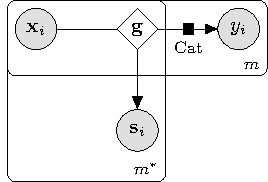
\includegraphics[width=0.35\textwidth]{figures/general_model}
\caption{Вероятностная модель в формате плоских нотаций.}
\label{fg:st:plate}
\end{figure}

На рис.~\ref{fg:st:plate} показан вид вероятностной модели в графовой нотации \DIFdelbegin \DIFdel{, }\DIFdelend для произвольной функции~$\mathbf{g}$. Для каждой реализации~$\mathbf{g}$ \DIFdelbegin \DIFdel{соответсвующий }\DIFdelend \DIFaddbegin \DIFadd{соответствующий }\DIFaddend блок требует \DIFdelbegin \DIFdel{уточнение}\DIFdelend \DIFaddbegin \DIFadd{уточнения}\DIFaddend . На рис~\ref{fg:ex:synt:plate} показана более подробная реализация в случае, когда модель~$\mathbf{g}$ это линейная модель.

\section{Обучение с учителем для задачи классификации и регрессии}
\subsection{Случай классификации}
Для задачи многоклассовой классификации рассматриваются \DIFdelbegin \DIFdel{следующие }\DIFdelend вероятностные предположения:
\begin{enumlist}
\label{st:class:1}
	\item рассматривается функция учителя $\mathbf{f}\in\mathfrak{F}_{\text{cl}}^{*}$~\eqref{eq:F:set:cl:priv};
	\item рассматривается функция ученика   \DIFdelbegin \DIFdel{следующего вида }\DIFdelend $\mathbf{g}\in\mathfrak{G}_{\text{cl}}$~\eqref{eq:G:set:cl};
	\item для истинных меток рассматривается категориальное распределение~$p\bigr(y|\mathbf{x}, \mathbf{g}\bigr) = \text{Cat}\bigr(\mathbf{g}\bigr(\mathbf{x}\bigr)\bigr)$, где $\mathbf{g}\bigr(\mathbf{x}\bigr)$ задает вероятность каждого класса;
	\item для меток учителя введем плотность распределения
\begin{gather}
\label{reg:dist}
\begin{aligned}
	p\bigr(\mathbf{s}|\mathbf{x}, \mathbf{g}\bigr) = C\prod_{k=1}^{K}g_k\bigr(\mathbf{x}\bigr)^{s^k},
\end{aligned}
\end{gather}
где~$g^k$ обозначает вероятность класса~$k$, которую предсказывает модель ученика, а~$s^k$~--- вероятность класса~$k$, которую предсказывает модель учителя.
\end{enumlist}
\begin{theorem}
\label{theorem:st:dist}
Пусть \DIFdelbegin \DIFdel{вероятнось }\DIFdelend \DIFaddbegin \DIFadd{вероятность }\DIFaddend каждого класса отделима от нуля и единицы, то есть для всех $k$ выполняется \DIFdelbegin \DIFdel{$1 > 1- \varepsilon > g_k\bigr(\mathbf{x}\bigr) > \varepsilon > 0,$ тогда }\DIFdelend \DIFaddbegin \DIFadd{условие
}\[\DIFadd{1 > 1- \varepsilon > g_k\bigr(\mathbf{x}\bigr) > \varepsilon > 0.
}\]
\DIFadd{Тогда }\DIFaddend при
\begin{gather}
C=\left(-1\right)^{K}\frac{K^{K/2}}{2^{K(K-1)/2}}\prod_{k=1}^{K}g_k\bigr(\mathbf{x}\bigr)\log g_k\bigr(\mathbf{x}\bigr)
\end{gather}
функция $p\bigr(\mathbf{s}|\mathbf{x}, \mathbf{g}\bigr)$ определенная в~\eqref{reg:dist} является плотностью распределения.
\end{theorem}
\begin{proof}
	Во-первых покажем, что для произвольного вектора ответов $\mathbf{s} \in \mathcal{S}_K$ выполняется $p\bigr(\mathbf{s}|\mathbf{x}, \mathbf{g}\bigr) \geq 0$. Заметим, что для всех~$k$ выполняется
	\DIFdelbegin \DIFdel{, что~$\log g_k\bigr(\mathbf{x}\bigr) < 0,$ тогда
}\begin{eqnarray*}
\DIFdel{\begin{aligned}
	C=\underbrace{\frac{K^{K/2}}{2^{K(K-1)/2}}}_{>0}\prod_{k=1}^{K}\underbrace{g_k\bigr(\mathbf{x}\bigr)}_{>\varepsilon}\underbrace{\left(-\log g_k\bigr(\mathbf{x}\bigr)\right)}_{>0} > 0,
\end{aligned}
}\end{eqnarray*}%DIFAUXCMD
\DIFdelend \DIFaddbegin \[\DIFadd{\log g_k\bigr(\mathbf{x}\bigr) < 0,}\]\DIFaddend  тогда
\DIFdelbegin \DIFdel{с }\DIFdelend \DIFaddbegin \begin{gather}
\DIFadd{\begin{aligned}
	C=\underbrace{\frac{K^{K/2}}{2^{K(K-1)/2}}}_{>0}\prod_{k=1}^{K}\underbrace{g_k\bigr(\mathbf{x}\bigr)}_{>\varepsilon}\underbrace{\left(-\log g_k\bigr(\mathbf{x}\bigr)\right)}_{>0} > 0.
\end{aligned}
}\end{gather}
\DIFadd{С }\DIFaddend учетом того, что~$g_k\bigr(\mathbf{x}\bigr) >0$ и~$C>0$ получаем, что $p\bigr(\mathbf{s}|\mathbf{x}, \mathbf{g}\bigr) \geq 0$.
	Во-вторых покажем, что интеграл по всему пространству ответов~$\mathcal{S}_K$ является конечным:
	\begin{gather}
	\label{theorem:st:dist:eq:1}
	\begin{aligned}
		\int_{\mathcal{S}_K}p\bigr(\mathbf{s}|\mathbf{x}, \mathbf{g}\bigr)ds &= \int_{\mathcal{S}_K}\prod_{k=1}^{K}g_k\bigr(\mathbf{x}\bigr)^{s^k}ds = \prod_{k=1}^{K}\int_{\mathcal{S}_K}g_k\bigr(\mathbf{x}\bigr)^{s^k}ds\\ 
		& = \prod_{k=1}^{K}\int_{0}^{1}\frac{r^{K-1}\sqrt{K}}{\left(K-1\right)!\sqrt{2^{K-1}}}g_k\bigr(\mathbf{x}\bigr)^{r}dr = \prod_{k=1}^{K}\underbrace{\frac{\sqrt{K}}{\left(K-1\right)!\sqrt{2^{K-1}}}}_{D}\int_{0}^{1}r^{K-1}g_k\bigr(\mathbf{x}\bigr)^{r}dr \\
		& = D^K\prod_{k=1}^{K} \int_{0}^{1}r^{K-1}\exp\bigr(r\log g_k\bigr(\mathbf{x}\bigr)\bigr)dr \\
		& = \left(-D\right)^K\prod_{k=1}^{K}\log g_k\bigr(\mathbf{x}\bigr)\left(\Gamma\bigr(K\bigr) - \Gamma\bigr(K, -\log g_k\bigr(\mathbf{x}\bigr)\bigr)\right) \\
		& = \left(-D\right)^K\left(K-1\right)!^K\prod_{k=1}^{K}\log g_k\bigr(\mathbf{x}\bigr)\left(1 -g_k\bigr(\mathbf{x}\bigr) \exp_{K-1}\bigr(-\log g_k\bigr(\mathbf{x}\bigr)\bigr)+g_k\bigr(\mathbf{x}\bigr)\right) \\
		& = \frac{\left(-\sqrt{K}\right)^K}{2^{K(K-1)/2}}\prod_{k=1}^{K}\log g_k\bigr(\mathbf{x}\bigr)\left(1 -g_k\bigr(\mathbf{x}\bigr) \exp_{K-1}\bigr(-\log g_k\bigr(\mathbf{x}\bigr)\bigr)+g_k\bigr(\mathbf{x}\bigr)\right) < \infty,
	\end{aligned}
	\end{gather}
где~$\Gamma\bigr(K\bigr)$ является гамма функцией, $\Gamma\bigr(K, -\log g_k\bigr(\mathbf{x}\bigr)\bigr)$ является неполной гамма функцией, $\exp_{n}\bigr(x\bigr)$ является суммой Тейлора из первых~$n$ слагаемых. В рамках приближенных расчетов будем считать, что $\exp_{n}\bigr(x\bigr)\approx\exp\bigr(x\bigr),$ тогда с учетом~\eqref{theorem:st:dist:eq:1} получаем
	\DIFdelbegin \DIFdel{:
	}\DIFdelend \begin{gather}
	\label{theorem:st:dist:eq:2}
	\begin{aligned}
		C\bigr(\mathbf{g}, \mathbf{x}\bigr) = \int_{\mathcal{S}_K}p\bigr(\mathbf{s}|\mathbf{x}, \mathbf{g}\bigr)ds \approx \left(-1\right)^{K}\frac{K^{K/2}}{2^{K(K-1)/2}}\prod_{k=1}^{K}g_k\bigr(\mathbf{x}\bigr)\log g_k\bigr(\mathbf{x}\bigr)
	\end{aligned}
	\end{gather}
\DIFdelbegin %DIFDELCMD < 

%DIFDELCMD < %%%
\DIFdelend Полученное выражение~\eqref{theorem:st:dist:eq:2} заканчивает доказательство теоремы.
\end{proof}

Из теоремы~\ref{theorem:st:dist} следует, что плотность введенная для меток учителя является плотностью распределения, следовательно можно воспользоваться выражением~\eqref{eq:st:12}.
Используя предположения~1)--4) и подставляя в~\eqref{eq:st:12} получаем  \DIFdelbegin \DIFdel{следующую }\DIFdelend оптимизационную задачу:
\begin{gather}
\label{eq:st:class:1}
\begin{aligned}
\hat{\mathbf{g}} = \arg\max_{\mathbf{g}\in \mathcal{G}} & \sum_{i\not\in \mathcal{I}}\sum_{k=1}^{K}y_i^k\log g_k\bigr(\mathbf{x}_i\bigr)\bigr|_{T=1} \\
&+ \left(1-\lambda\right)\sum_{i\in \mathcal{I}}\sum_{k=1}^{K}y_i^k\log g_k\bigr(\mathbf{x}_i\bigr)\bigr|_{T=1} + \lambda\sum_{i\in \mathcal{I}}\sum_{k=1}^{K}s_{i,k}\log g_k\bigr(\mathbf{x}_i\bigr)\bigr|_{T=T_0} \\
&+ \lambda \sum_{i\in \mathcal{I}}\sum_{k=1}^{K}\left(\log g_k\bigr(\mathbf{x}_i\bigr)\bigr|_{T=T_0} + \log\log\frac{1}{g_k\bigr(\mathbf{x}_i\bigr)}\bigr|_{T=T_0}\right),
\end{aligned}
\end{gather}
где выражение $\cdot\bigr|_{T=t}$ обозначает, что в предыдущую функцию $\text{softmax}$ требуется подставить значение температуры~$T$ равное\DIFdelbegin \DIFdel{некоторому значению}\DIFdelend ~$t$.

Проанализировав выражение~\eqref{eq:st:class:1} получаем, что первые три слагаемые совпадают со слагаемыми в выражении~\eqref{eq:hinton:1} при~$\mathcal{I} = \{1, \cdots, m\},$ и $\lambda=\frac{1}{2}$, а \DIFdelbegin \DIFdel{третье }\DIFdelend \DIFaddbegin \DIFadd{четвертое }\DIFaddend слагаемое является некоторым регуляризатором, который получен из вида распределения. \DIFdelbegin %DIFDELCMD < 

%DIFDELCMD < %%%
\DIFdelend Анализируя первые три слагаемых в выражении~\eqref{eq:st:class:1} \DIFdelbegin \DIFdel{получаем, что }\DIFdelend при~$T_0 = 1$ получаем сумму \DIFdelbegin \DIFdel{кросс энтропий }\DIFdelend \DIFaddbegin \DIFadd{кросс-энтропий }\DIFaddend между двумя распределениями для каждого объекта:
\begin{enumlist}
	\item первое распределение\DIFaddbegin \DIFadd{~--- }\DIFaddend это выпуклая комбинация с \DIFdelbegin \DIFdel{весом}\DIFdelend \DIFaddbegin \DIFadd{весами}\DIFaddend ~$1-\lambda$ и $\lambda$ \DIFdelbegin \DIFdel{: }\DIFdelend распределения\DIFdelbegin \DIFdel{задаваемое }\DIFdelend \DIFaddbegin \DIFadd{, задаваемого }\DIFaddend метками объектов~$\text{Cat}\bigr(\mathbf{y}\bigr)$ и распределения\DIFaddbegin \DIFadd{, }\DIFaddend задаваемого моделью учителя~$\text{Cat}\bigr(\mathbf{s}\bigr)$
	\item второе распределение\DIFaddbegin \DIFadd{~--- }\DIFaddend это распределение\DIFaddbegin \DIFadd{, }\DIFaddend задаваемое моделью ученика~$\text{Cat}\bigr(\mathbf{g}\bigr(\mathbf{x}\bigr)\bigr)$.
\end{enumlist}
\DIFdelbegin \DIFdel{Получаем, что }\DIFdelend \DIFaddbegin \DIFadd{Следовательно, }\DIFaddend модель ученика восстанавливает плотность не исходных меток, а новую плотность, которая является выпуклой комбинаций плотности исходных меток и меток учителя.
\subsection{Случай регрессии}
Для задачи регрессии рассматриваются \DIFdelbegin \DIFdel{следующие }\DIFdelend вероятностные предположения:
\begin{enumlist}
	\item рассматривается функция учителя~$\mathbf{f}\in\mathfrak{F}_{\text{rg}}^{*}$\DIFdelbegin \DIFdel{:
	}\DIFdelend \DIFaddbegin \DIFadd{,
	}\DIFaddend \begin{gather}
	\label{eq:F:set:priv}
	\begin{aligned}
	\mathfrak{F}_{\text{rg}}^* = \left\{\mathbf{f}| \mathbf{f} = \mathbf{v}^*\bigr(\mathbf{x}^*\bigr), \quad \mathbf{v}^*: \mathbb{R}^{n^*} \to \mathbb{R} \right\},
	\end{aligned}
	\end{gather}
	где~$\mathbf{v}^*$~--- это дифференцируемая параметрическая функция;
	\item рассматривается функция ученика~$\mathbf{g}\in\mathfrak{G}_{\text{rg}}$\DIFdelbegin \DIFdel{:
}\DIFdelend \DIFaddbegin \DIFadd{,
}\DIFaddend \begin{gather}
\label{eq:G:set:rg}
\mathfrak{G}_{\text{rg}} = \left\{\mathbf{g}| \mathbf{g} = \mathbf{z}\bigr(\mathbf{x}\bigr), \quad \mathbf{z}: \mathbb{R}^n \to \mathbb{R}^K \right\},
\end{gather}
где~$\mathbf{z}$~--- это дифференцируемая параметрическая функция;
	\item истинные метки имеют нормальное распределение
	\begin{gather}
		p\bigr(y|\mathbf{x}, \mathbf{g}\bigr) = \mathcal{N}\bigr(y|\mathbf{g}\bigr(\mathbf{x}\bigr), \sigma\bigr);
	\end{gather}
	\item метки учителя \DIFdelbegin \DIFdel{распределены
	}\DIFdelend \DIFaddbegin \DIFadd{имеют распределение
	}\DIFaddend \begin{gather}
		p\bigr(s| \mathbf{x}, \mathbf{g}\bigr) = \mathcal{N}\bigr(s|\mathbf{g}\bigr(\mathbf{x}\bigr), \sigma_s\bigr)\DIFdelbegin \DIFdel{;
	}\DIFdelend \DIFaddbegin \DIFadd{.
	}\DIFaddend \end{gather}
\end{enumlist}

Используя предположения~1)--4) и подставляя в~\eqref{eq:st:12} получаем \DIFdelbegin \DIFdel{следующую }\DIFdelend оптимизационную задачу:
\begin{gather}
\label{eq:st:reg:1}
\begin{aligned}
\hat{g} = \arg\min_{g\in \mathcal{G}} & \sum_{i\not\in \mathcal{I}}\sigma^2\left(y_i-\mathbf{g}\bigr(\mathbf{x}_i\bigr)\right)^2 \\
&+ \left(1-\lambda\right)\sum_{i\in \mathcal{I}}\sigma^2\left(y_i-\mathbf{g}\bigr(\mathbf{x}_i\bigr)\right)^2 + \lambda\sum_{i\in \mathcal{I}}\sigma_s^2\left(s_i-\mathbf{g}\bigr(\mathbf{x}_i\bigr)\right)^2.
\end{aligned}
\end{gather}
Выражение~\eqref{eq:st:reg:1} записано с точностью до аддитивной константы относительно~$\mathbf{g}$. 

\begin{theorem}
\label{theorem:st:reg}
Пусть множество~$\mathcal{G}$ описывает класс линейных функций вида~$\mathbf{g}\bigr(\mathbf{x}\bigr) = \mathbf{w}^{\mathsf{T}}\mathbf{x}.$ Тогда решение оптимизационной задачи~\eqref{eq:st:reg:1} эквивалентно решению \DIFdelbegin \DIFdel{следующей }\DIFdelend задачи линейной регрессии:
\begin{gather}
\label{eq:st:reg:th:st:1}
\DIFdelbegin %DIFDELCMD < \begin{aligned}
%DIFDELCMD < \mathbf{y''} = \mathbf{X}\mathbf{w} + \bm{\varepsilon},~\bm{\varepsilon} \sim \mathcal{N}\bigr(\mathbf{0}, \bm{\Sigma}\bigr),
%DIFDELCMD < \end{aligned}%%%
\DIFdelend \DIFaddbegin \begin{aligned}
\mathbf{y''} = \mathbf{X}\mathbf{w} + \bm{\varepsilon},\qquad \bm{\varepsilon} \sim \mathcal{N}\bigr(\mathbf{0}, \bm{\Sigma}\bigr),
\end{aligned}\DIFaddend 
\end{gather}
где $\bm{\Sigma}^{-1}=\text{diag}\bigr(\bm{\sigma'}\bigr)$ и $\mathbf{y''}$ имеют \DIFdelbegin \DIFdel{следующий }\DIFdelend вид:
\begin{gather}
\label{eq:st:reg:th:st:2}
\begin{aligned}
\sigma'_{i} &= \begin{cases}
\sigma^2,~\text{если}~i \not \in \mathcal{I}\\
\left(1-\lambda\right)\sigma^2+\lambda\sigma_s^2,~\text{иначе}\\
\end{cases}, \\
\mathbf{y''} &= \bm{\Sigma}\mathbf{y'},\\
y'_i &= \begin{cases}
\sigma^2y_i,~\text{если}~i \not \in \mathcal{I}\\
\left(1-\lambda\right)\sigma^2y_i+\lambda\sigma_s^2s_i,~\text{иначе}\\
\end{cases}.
\end{aligned}
\end{gather}
\end{theorem}
\begin{proof}
\DIFdelbegin \DIFdel{Обозначеним}\DIFdelend \DIFaddbegin \DIFadd{Обозначим}\DIFaddend ~$\mathbf{a}_{\mathcal{J}} = [a_i| i \in \mathcal{J}]^{\mathsf{T}},$ где~$\mathbf{a}$ произвольный вектор, а $\mathcal{J}$ произвольное \DIFdelbegin \DIFdel{не пустое }\DIFdelend \DIFaddbegin \DIFadd{непустое }\DIFaddend индексное множество. Подвектор вектора ответов~$\mathbf{y}$, для элементов которого доступна привилегированная информация обозначим $\mathbf{y}_{\mathcal{I}} = [y_i| i \in \mathcal{I}]^{\mathsf{T}}$. Аналогично обозначим матрицу~$\mathbf{X}_\mathcal{I}=[\mathbf{x}_{i}| i \in \mathcal{I}]^{\mathsf{T}}$.

В случае линейной модели~$\mathbf{g}\bigr(\mathbf{x}\bigr) = \mathbf{w}^{\mathsf{T}}\mathbf{x}$ выражение \eqref{eq:st:reg:1} принимает вид:
\begin{gather}
\label{eq:st:reg:2}
\begin{aligned}
\hat{\mathbf{w}} = \arg\min_{\mathbf{w}\in \mathcal{W}} &~ \sigma^2\left(\mathbf{y}_{\bar{\mathcal{I}}}-\mathbf{X}_{\bar{\mathcal{I}}}\mathbf{w}\right)^{\mathsf{T}}\left(\mathbf{y}_{\bar{\mathcal{I}}}-\mathbf{X}_{\bar{\mathcal{I}}}\mathbf{w}\right) \\
&+ \sigma^2\left(1-\lambda\right)\left(\mathbf{y}_{\mathcal{I}}-\mathbf{X}_{\mathcal{I}}\mathbf{w}\right)^{\mathsf{T}}\left(\mathbf{y}_{\mathcal{I}}-\mathbf{X}_{\mathcal{I}}\mathbf{w}\right) + \sigma^2_s\lambda\left(\mathbf{s}_{\mathcal{I}}-\mathbf{X}_{\mathcal{I}}\mathbf{w}\right)^{\mathsf{T}}\left(\mathbf{s}_{\mathcal{I}}-\mathbf{X}_{\mathcal{I}}\mathbf{w}\right).
\end{aligned}
\end{gather}

Раскроем скобки и сгруппируем:
\begin{gather}
\label{eq:st:reg:3}
\begin{aligned}
\hat{\mathbf{w}} = \arg\min_{\mathbf{w}\in \mathcal{W}} &~ \sigma^2\left(\mathbf{w}^{\mathsf{T}}\mathbf{X}^{\mathsf{T}}_{\bar{\mathcal{I}}}\mathbf{X}_{\bar{\mathcal{I}}}\mathbf{w} - 2\mathbf{y}^{\mathsf{T}}_{\bar{\mathcal{I}}}\mathbf{X}_{\bar{\mathcal{I}}}\mathbf{w}\right) \\
&+ \left(1-\lambda\right)\sigma^2\left(\mathbf{w}^{\mathsf{T}}\mathbf{X}^{\mathsf{T}}_{\mathcal{I}}\mathbf{X}_{\mathcal{I}}\mathbf{w}- 2\mathbf{y}^{\mathsf{T}}_{\mathcal{I}}\mathbf{X}_{\mathcal{I}}\mathbf{w}\right) + \lambda\sigma^2_s\left(\mathbf{w}^{\mathsf{T}}\mathbf{X}^{\mathsf{T}}_{\mathcal{I}}\mathbf{X}_{\mathcal{I}}\mathbf{w}- 2\mathbf{s}^{\mathsf{T}}_{\mathcal{I}}\mathbf{X}_{\mathcal{I}}\mathbf{w}\right)
\end{aligned}
\end{gather}
Продифференцируем выражение, приравняем к нулю и сгруппируем элементы:
\begin{gather}
\label{eq:st:reg:4}
\begin{aligned}
\left(\sigma^{2}\mathbf{X}^{\mathsf{T}}_{\bar{\mathcal{I}}}\mathbf{X}_{\bar{\mathcal{I}}} + \left(1-\lambda\right)\sigma^2\mathbf{X}^{\mathsf{T}}_{\mathcal{I}}\mathbf{X}_{\mathcal{I}} + \lambda\sigma^{2}_s\mathbf{X}^{\mathsf{T}}_{\mathcal{I}}\mathbf{X}_{\mathcal{I}}\right) \mathbf{w} =& 2\sigma^2\mathbf{X}^{\mathsf{T}}_{\bar{\mathcal{I}}}\mathbf{y}_{\bar{\mathcal{I}}} \\
&+ 2\left(1-\lambda\right)\sigma^2\mathbf{X}^{\mathsf{T}}_{\mathcal{I}}\mathbf{y}_{\mathcal{I}} + 2\lambda\sigma_s^2\mathbf{X}^{\mathsf{T}}_{\mathcal{I}}\mathbf{s}_{\mathcal{I}}.
\end{aligned}
\end{gather}
Воспользуемся \DIFdelbegin \DIFdel{следующими }\DIFdelend равенствами:
\begin{gather}
\label{eq:st:reg:simp}
\begin{aligned}
\sigma^{2}\mathbf{X}^{\mathsf{T}}_{\bar{\mathcal{I}}}\mathbf{X}_{\bar{\mathcal{I}}} + \left(1-\lambda\right)\sigma^2\mathbf{X}^{\mathsf{T}}_{\mathcal{I}}\mathbf{X}_{\mathcal{I}} + \lambda\sigma^{2}_s\mathbf{X}^{\mathsf{T}}_{\mathcal{I}}\mathbf{X}_{\mathcal{I}} &= \mathbf{X}^{\mathsf{T}}\bm{\Sigma}^{-1}\mathbf{X},\\
2\sigma^2\mathbf{X}^{\mathsf{T}}_{\bar{\mathcal{I}}}\mathbf{y}_{\bar{\mathcal{I}}} + 2\left(1-\lambda\right)\sigma^2\mathbf{X}^{\mathsf{T}}_{\mathcal{I}}\mathbf{y}_{\mathcal{I}} + 2\lambda\sigma_s^2\mathbf{X}^{\mathsf{T}}_{\mathcal{I}}\mathbf{s}_{\mathcal{I}} &= 2\mathbf{X}\mathbf{y'},
\end{aligned}
\end{gather}
где~$\bm{\Sigma}$ и~$\mathbf{y'}$ из условия задачи~\eqref{eq:st:reg:th:st:2}.

Подставляя~\eqref{eq:st:reg:simp} в~\eqref{eq:st:reg:4} получаем:
\begin{gather}
\label{eq:st:reg:5}
\begin{aligned}
\mathbf{w} = 2\left(\mathbf{X}^{\mathsf{T}}\bm{\Sigma}^{-1}\mathbf{X}\right)^{-1}\mathbf{X}\bm{\Sigma}^{-1}\mathbf{y''},
\end{aligned}
\end{gather}
что \DIFdelbegin \DIFdel{соответсвует }\DIFdelend \DIFaddbegin \DIFadd{соответствует }\DIFaddend решению задачи~\eqref{eq:st:reg:th:st:1}.
\end{proof}

Теорема~\ref{theorem:st:reg} показывает, что обучения с учителем для задачи регрессии можно свести к классической \DIFdelbegin \DIFdel{задачи }\DIFdelend \DIFaddbegin \DIFadd{задаче }\DIFaddend оптимизации для задачи линейной регрессии.

\section{Вычислительный эксперимент}
Проводится вычислительный эксперимент для анализа \DIFdelbegin \DIFdel{качества }\DIFdelend моделей, которые получены путем дистилляции модели учителя в модель ученика. Как показано в теореме~\ref{theorem:st:reg} задачу регрессии с учителем можно свести к \DIFdelbegin \DIFdel{задачи }\DIFdelend \DIFaddbegin \DIFadd{задаче }\DIFaddend регрессии без учителя, поэтому в эксперименте \DIFdelbegin \DIFdel{более подробно }\DIFdelend рассматривается \DIFaddbegin \DIFadd{только }\DIFaddend случай классификации. Во всех частях вычислительного эксперимента для поиска оптимальных параметров нейросетей использовался градиентный метод оптимизации \DIFdelbegin \DIFdel{Адам}\DIFdelend \DIFaddbegin \DIFadd{Adam}\DIFaddend ~\cite{kingma2014}.
\subsection{Выборка FashionMNIST}
В данной части проводится эксперимент для задачи классификации для выборки FashionMNIST~\cite{fashionmnist}. В качестве модели учителя~$\mathbf{f}$ рассматривается \DIFdelbegin \DIFdel{модель нейросети }\DIFdelend \DIFaddbegin \DIFadd{нейросеть }\DIFaddend с двумя сверточными слоями и с тремя полносвязными слоями, в качестве функции активации рассматривается ReLu. Модель учителя содержит~$~30$ тысяч обучаемых параметров. В качестве модели ученика рассматривается модель логистической регрессии для многоклассовой классификации. Модель ученика содержит~$7850$ обучаемых параметров.

\begin{figure}[h!t]\center
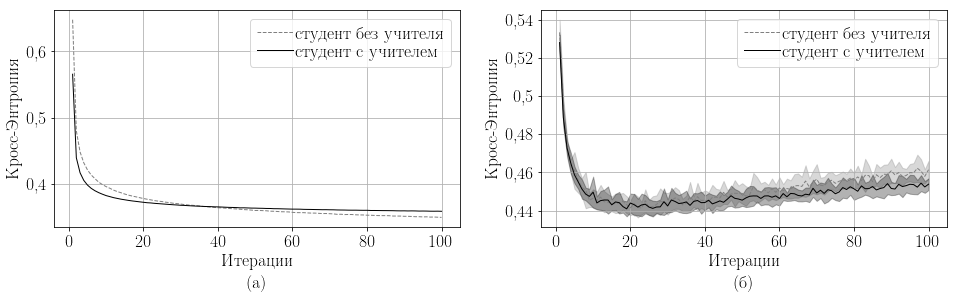
\includegraphics[width=1\textwidth]{figures/mnist_loss}
\caption{Зависимость \DIFdelbeginFL \DIFdelFL{кросс--этропии }\DIFdelendFL \DIFaddbeginFL \DIFaddFL{кросс-энтропии }\DIFaddendFL между истинными метками и предсказанными учеников вероятностями классов: a) на обучающей выборке; b) на тестовой выборке.}
\label{fg:ex:fashionmnist:loss}
\end{figure}

На рис.~\ref{fg:ex:fashionmnist:loss} показан график зависимости кросс--энтропии между истинными метками объектов и вероятностями, которые предсказывает модель ученика. На графике сравнивается \DIFdelbegin \DIFdel{моделя}\DIFdelend \DIFaddbegin \DIFadd{модель}\DIFaddend , которая обучалась без учителя (в задаче оптимизации~\eqref{eq:st:class:1} присутствует только первое слагаемое) с моделью, которая была получена путем дистилляции модели нейросети в линейную модель. \DIFdelbegin \DIFdel{На графике }\DIFdelend \DIFaddbegin \DIFadd{Из графика }\DIFaddend видно, что обе модели начинают \DIFdelbegin \DIFdel{переобучатся }\DIFdelend \DIFaddbegin \DIFadd{переобучаться }\DIFaddend после 30-й итерации\DIFdelbegin \DIFdel{, но }\DIFdelend \DIFaddbegin \DIFadd{. Но }\DIFaddend модель, которая получена путем дистилляции\DIFdelbegin \DIFdel{переобувается }\DIFdelend \DIFaddbegin \DIFadd{, переобучается }\DIFaddend не так быстро\DIFdelbegin \DIFdel{, что следует из того, что }\DIFdelend \DIFaddbegin \DIFadd{: }\DIFaddend ошибка на тестовой выборке растет медленней, а на обучающей выборке падает также медленней.


\subsection{Синтетический эксперимент}
Проанализируем модель на синтетической выборке. Выборка \DIFdelbegin \DIFdel{построенная }\DIFdelend \DIFaddbegin \DIFadd{построена }\DIFaddend следующим образом:
\begin{gather}
\begin{aligned}
\mathbf{W} &= \left[\mathcal{N}\bigr(w_{jk}|0, 1\bigr)\right]_{n\times K}, \quad &\mathbf{X} &= \left[\mathcal{N}\bigr(x_{ij}|0, 1\bigr)\right]_{m\times n}, \\
 \mathbf{S} &= \text{softmax}\left(\mathbf{XW}\right), \quad &\mathbf{y} &= \left[\text{Cat}\bigr(y_i| \mathbf{s}_i\bigr)\right],
\end{aligned}
\end{gather}
где функция~$\text{softmax}$ берется построчно. Строки матрицы~$\mathbf{S}$ будем рассматривать как предсказание учителя, то есть учитель знает истинные вероятности каждого класса. На рис.~\ref{fg:ex:synt:plate} показана вероятностная модель в графовой нотации. В эксперименте число признаков~$n=10$, число классов~$K=3$, для обучения было сгенерировано~$m_{\text{train}}=1000$ и~$m_{\text{test}}=100$ объектов.

На рис.~\ref{fg:ex:synt:distr:real} показано распределение по классам для\DIFdelbegin \DIFdel{каждого объекта }\DIFdelend \DIFaddbegin \DIFadd{~$20$ объектов из }\DIFaddend обучающей выборки. \DIFaddbegin \DIFadd{Каждому столбцу на графике соответствует объект, а каждой строке соответствует вероятность класса. }\DIFaddend Видно, что \DIFdelbegin \DIFdel{все классы являются равновероятными. }\DIFdelend \DIFaddbegin \DIFadd{для каждого рассмотренного объекта вероятности разных классов близки. Получается, что если в качестве истинных меток взять класс с максимальной вероятностью, то выборка будет сильно зашумленной и модель будет описывать эти данные некорректно.
}\DIFaddend 

Построим в качестве ученика \DIFdelbegin \DIFdel{простую }\DIFdelend линейную модель, которая минимизирует крос--энтропийную (первое слагаемое в формуле~\eqref{eq:st:class:1}). Представление данной модели в виде графовой модели показано на рис.~\ref{fg:ex:synt:plate}.

\begin{figure}[h!t]\center
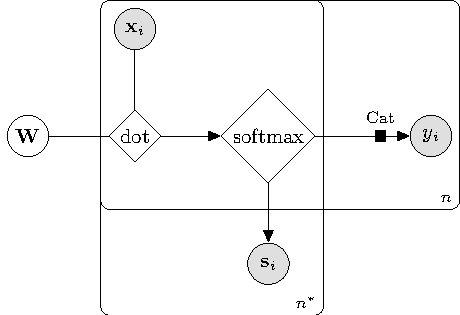
\includegraphics[width=0.35\textwidth]{figures/linear_model}
\caption{Вероятностная модель используемая в синтетическом эксперименте.}
\label{fg:ex:synt:plate}
\end{figure}

\begin{figure}[h!t]\center
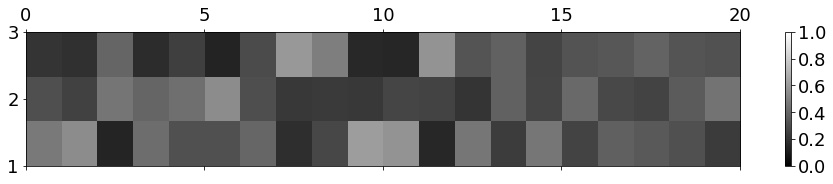
\includegraphics[width=1\textwidth]{figures/syn_real_distr}
\caption{Истинное распределение  объектов по классам.}
\label{fg:ex:synt:distr:real}
\end{figure}


На рис.~\ref{fg:ex:synt:distr:without} показано распределение вероятностей классов, которое предсказала модель. Видно, что \DIFdelbegin \DIFdel{данное }\DIFdelend \DIFaddbegin \DIFadd{полученное }\DIFaddend распределение \DIFdelbegin \DIFdel{является }\DIFdelend не соответствует истинному, так как модель сосредотачивает всю вероятность в одном классе.

\begin{figure}[h!t]\center
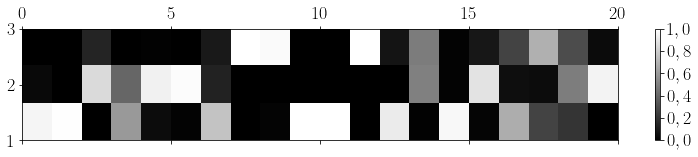
\includegraphics[width=1\textwidth]{figures/syn_without_teacher_distr}
\caption{Распределение предсказанное моделью без использования информации об истинном распределение на классах.}
\label{fg:ex:synt:distr:without}
\end{figure}

\begin{figure}[h!t]\center
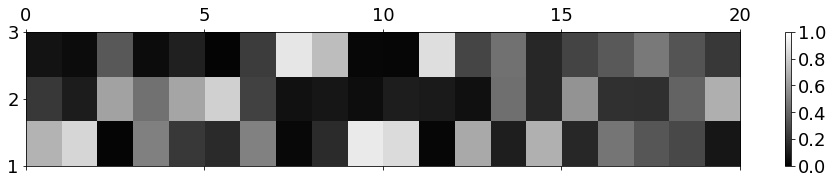
\includegraphics[width=1\textwidth]{figures/syn_with_teacher_distr}
\caption{Распределение\DIFaddbeginFL \DIFaddFL{, }\DIFaddendFL предсказанное моделью \DIFdelbeginFL \DIFdelFL{c использования }\DIFdelendFL \DIFaddbeginFL \DIFaddFL{с использованием }\DIFaddendFL информации об истинном распределение на классах.}
\label{fg:ex:synt:distr:with}
\end{figure}

\begin{figure}[h!t]\center
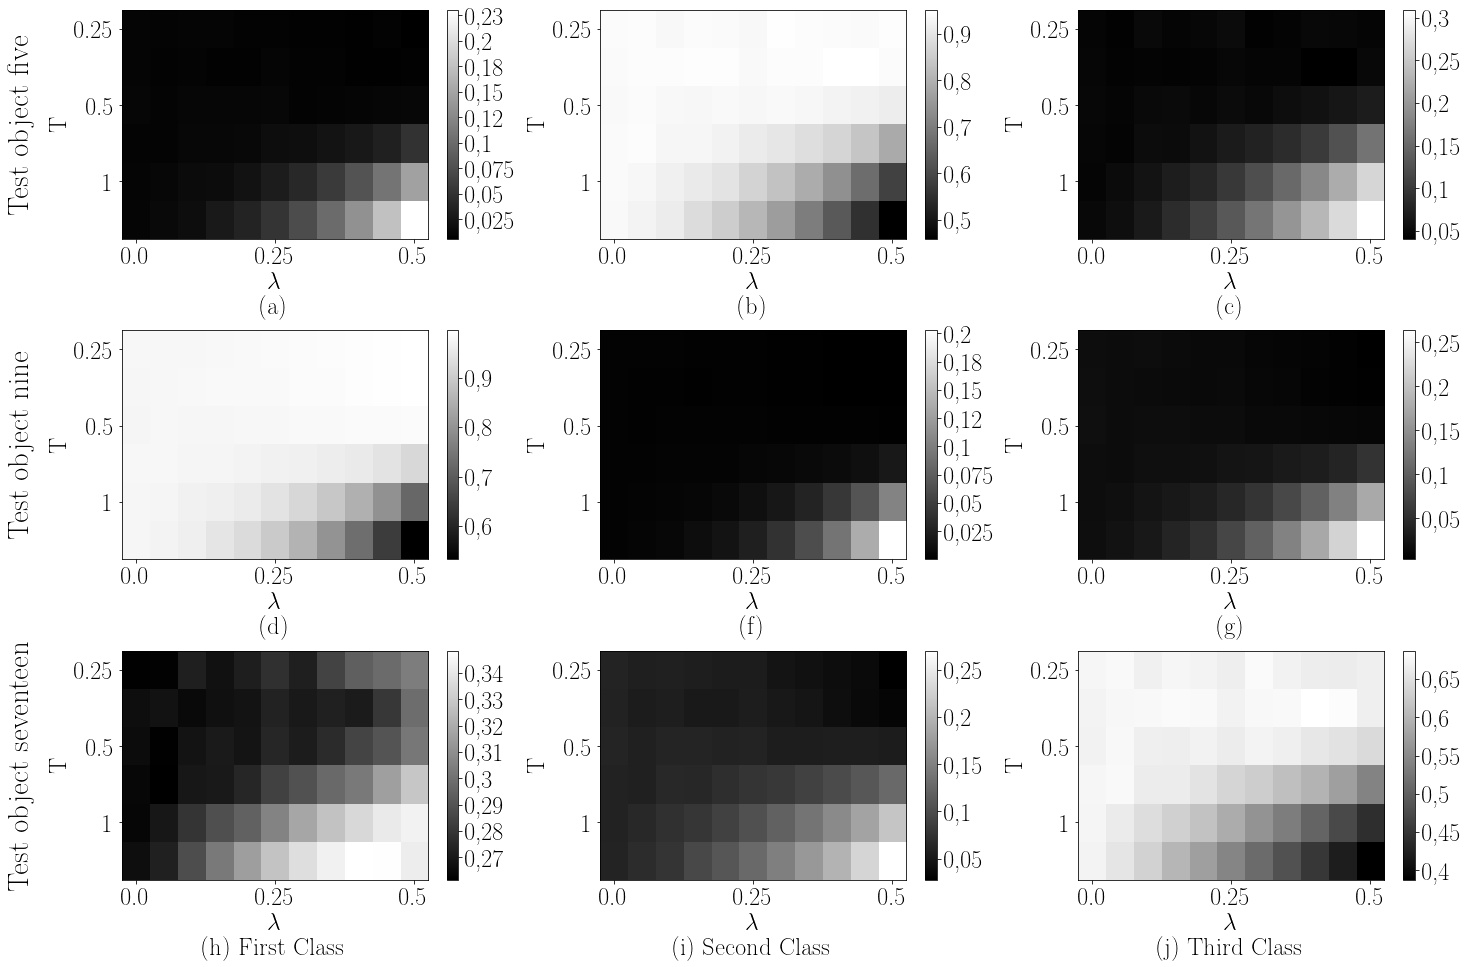
\includegraphics[width=1\textwidth]{figures/syn_T_lambda}
\caption{\DIFdelbeginFL \DIFdelFL{Вероятности }\DIFdelendFL \DIFaddbeginFL \DIFaddFL{Иллюстрация распределения вероятности предсказания }\DIFaddendFL классов \DIFdelbeginFL \DIFdelFL{для разных объектов}\DIFdelendFL \DIFaddbeginFL \DIFaddFL{при различных значениях~$\lambda$ и $T$}\DIFaddendFL .}
\label{fg:ex:synt:distr:lambda_T}
\end{figure}

Рассмотрим модель, которая учитывает информацию \DIFdelbegin \DIFdel{о }\DIFdelend \DIFaddbegin \DIFadd{об }\DIFaddend истинных распределениях на классах для каждого объекта. Для этого будем минимизировать первые три слагаемых в формуле~\eqref{eq:st:class:1}, при~$T_0=1$ и~$\lambda=0{,}75$. В качестве меток учителя~$s_{i,k}$ использовались истинные вероятности для каждого класса для данного объекта. На рис\DIFaddbegin \DIFadd{.}\DIFaddend ~\ref{fg:ex:synt:distr:with} показано распределение, которое дала модель\DIFdelbegin \DIFdel{в }\DIFdelend \DIFaddbegin \DIFadd{. В }\DIFaddend данном случае, видно, что распределения являются сглаженными и концентрации всей вероятности в одном классе не наблюдается.

Заметим, что в данном примере предполагается, что модель учителя учитывает не только метки классов, а и распределение на метках классов, в то время как в выборке~\DIFdelbegin \DIFdel{$\mathcal{D} = \{\mathbf{X}, \mathbf{y}\},$ }\DIFdelend \DIFaddbegin \DIFadd{$\{\mathbf{X}, \mathbf{y}\},$ }\DIFaddend имеются только точечные оценки в виде \DIFdelbegin \DIFdel{меткок}\DIFdelend \DIFaddbegin \DIFadd{меток}\DIFaddend . 

В данном примере используются истинные распределения в качестве предсказаний учителя, но их можно заменить предсказаниями модели учителя, которая предсказывает не только сами меток, а и их распределение для каждого объекта.

На рис.~\ref{fg:ex:synt:distr:lambda_T} показана зависимость вероятности верного класса от температуры~$T$ и параметра доверия~$\lambda$ для одного из объекта из тестовой выборке. \DIFdelbegin \DIFdel{Видно}\DIFdelend \DIFaddbegin \DIFadd{На рисунке видно}\DIFaddend , что \DIFaddbegin \DIFadd{изменение температуры~$T$ влечет изменение концентрации вероятностной меры. При уменьшении параметра температуры к нулю, получаем, что вероятность одного из классов становиться близко к единице, а остальных близко к нулю. С другой стороны }\DIFaddend при \DIFdelbegin \DIFdel{увеличении темпертуры }\DIFdelend \DIFaddbegin \DIFadd{увеличения параметра температуры вероятности классов сглаживаются и }\DIFaddend распределение \DIFdelbegin \DIFdel{на классас }\DIFdelend \DIFaddbegin \DIFadd{классов для каждого объекта }\DIFaddend становится \DIFdelbegin \DIFdel{более равномерным}\DIFdelend \DIFaddbegin \DIFadd{близким к равномерному}\DIFaddend .

\DIFaddbegin \DIFadd{В таблице~\ref{tb:ce:1} в колонке ``Кросс-Энтропийная ошибка с реальными вероятностями'' показано сравнение кросс-энтропии в случае, если в качестве истинных вероятностей меток рассмотреть не onehot-кодированные вероятности классов, а истинные вероятности:
}\begin{gather}
\DIFadd{\label{eq:ce:1}
\begin{aligned}
\mathcal{L}_{\text{real}}\bigr(\mathbf{g}\bigr) = - \sum_{i=1}^{m}\sum_{k=1}^{K}s_{i}^{k}\log g_k\bigr(\mathbf{x}_i\bigr),
\end{aligned}
}\end{gather}
\DIFadd{где~$\mathbf{g}$ модель ученика. Видно, что модель с учителем лучше аппроксимирует истинные вероятности классов. Также в таблице~\ref{tb:ce:1} представлено среднее значение разницы максимальной вероятности с минимальной вероятностью для каждого объекта:
}\begin{gather}
\DIFadd{\label{eq:ce:2}
\begin{aligned}
\mathcal{L}_{\text{maxmin}}\bigr(\mathbf{g}\bigr) = \frac{1}{m}\sum_{i=1}^{m}\left(\max_{k}g_k\bigr(\mathbf{x}_i\bigr) -  \min_{k}g_k\bigr(\mathbf{x}_i\bigr)\right),
\end{aligned}
}\end{gather}
\DIFadd{Видно, что модель учителя имеет меньшую разницу между вероятностями классов, то есть вероятности классов не концентрируются в одном классе.
}

\DIFaddend \subsection{Выборка Twitter Sentiment Analysis}
В данной части проводится эксперимент на выборке Twitter Sentiment Analysis. Данная выборка содержит короткие сообщения, для которых \DIFdelbegin \DIFdel{нужно }\DIFdelend \DIFaddbegin \DIFadd{требуется }\DIFaddend предсказать эмоциональный окрас: содержит твит позитивный окрас или негативный. Выборка разделена на~$1{,}18$ миллиона твитов для обучения и~$0{,}35$ миллиона твитов для тестирования. В твитах была выполнена \DIFdelbegin \DIFdel{следующая }\DIFdelend предобработка: \DIFdelbegin %DIFDELCMD < \begin{itemize}
%DIFDELCMD < 	\item %%%
\DIFdelend все твиты были переведены в нижний регистр; \DIFdelbegin %DIFDELCMD < \item %%%
\DIFdelend все никнеймы вида~``@andrey'' были заменены на токен ``name''; \DIFdelbegin %DIFDELCMD < \item %%%
\DIFdelend все цифры были заменены на токен ``number''.
\DIFdelbegin %DIFDELCMD < \end{itemize}
%DIFDELCMD < %%%
\DIFdelend \DIFaddbegin 

\DIFaddend Результаты данной части эксперимента показаны в табл.~\ref{tb:ce:1}. В качестве модели учителя использовалась модель Bi-LSTM с \DIFdelbegin \DIFdel{~$170$ тысячами параметров для обучения}\DIFdelend \DIFaddbegin \DIFadd{линейным слоем на выходе}\DIFaddend . В качестве \DIFdelbegin \DIFdel{эмбедингов }\DIFdelend \DIFaddbegin \DIFadd{векторного представления токенов }\DIFaddend обучалась матрица \DIFaddbegin \DIFadd{параметров в которой каждая строка соответствует токену }\DIFaddend из \DIFaddbegin \DIFadd{обучающей выборки. Суммарное число обучаемых параметров модели учителя составляет более}\DIFaddend ~$30$ миллионов\DIFdelbegin \DIFdel{параметров в единой процедуре с моделью BI-LSTM}\DIFdelend . Обученная модель \DIFdelbegin \DIFdel{предсказывает с точностью}\DIFdelend \DIFaddbegin \DIFadd{учителя имеет точность предсказания}\DIFaddend ~$0{,}835$. В качестве модели ученика рассматривается \DIFaddbegin \DIFadd{линейная }\DIFaddend модель с $1538$ параметрами, \DIFdelbegin \DIFdel{но }\DIFdelend \DIFaddbegin \DIFadd{где }\DIFaddend в качестве \DIFdelbegin \DIFdel{эмбедингов }\DIFdelend \DIFaddbegin \DIFadd{векторного представления предложения }\DIFaddend рассматривается \DIFdelbegin \DIFdel{переобученная модель BERT }\DIFdelend \DIFaddbegin \DIFadd{выход предобученной модели BERT с размерностью векторного пространства~$768$. Признаковое описания модели учителя и модели ученика различаются}\DIFaddend . \DIFaddbegin \DIFadd{Модель учителя в качестве признакового описания рассматривается исходные слова в предложении. Модель ученика в качестве признакового описания использует готовое векторное представление предложения, которое получено при помощи модели BERT. В табл.~\ref{tb:ce:1} показано качество модели ученика с использованием предсказания модели учителя и без него.
}\DIFaddend 

Программное обеспечение для проведения экспериментов и проверки результатов находится в~\cite{Code2020}.

\section{Заключение}
\begin{table}[]
\caption{Сводная таблица результатов вычислительного эксперимента.}
\label{tb:ce:1}
\begin{center}
\DIFdelbeginFL %DIFDELCMD < \begin{tabular}{|l|l|c|c|c|}
%DIFDELCMD < \hline
%DIFDELCMD < \multicolumn{1}{|c|}{Dataset} & \multicolumn{1}{c|}{Model} & %%%
\DIFdelFL{CrossEntropyLoss      }%DIFDELCMD < & %%%
\DIFdelFL{Accuracy    }%DIFDELCMD < &   %%%
\DIFdelFL{StudentSize   }%DIFDELCMD < \\ \hline
%DIFDELCMD < \multirow{2}{*}{FashionMnist} & %%%
\DIFdelFL{without teacher    }%DIFDELCMD < &  %%%
\DIFdelFL{$0{,}461 \pm 0{,}005$ }%DIFDELCMD < & %%%
\DIFdelFL{$0{,}841\pm 0{,}002$ }%DIFDELCMD < & %%%
\DIFdelFL{7850 }%DIFDELCMD < \\ \cline{2-5} 
%DIFDELCMD <                               & %%%
\DIFdelFL{with teacher       }%DIFDELCMD < & %%%
\DIFdelFL{$0{,}453 \pm 0{,}003$ }%DIFDELCMD < & %%%
\DIFdelFL{$0{,}842 \pm 0{,}002$ }%DIFDELCMD < & %%%
\DIFdelFL{7850}%DIFDELCMD < \\ \hline
%DIFDELCMD < \multirow{2}{*}{Synthetic}    & %%%
\DIFdelFL{without teacher    }%DIFDELCMD < & %%%
\DIFdelFL{$0{,}225 \pm 0{,}002$ }%DIFDELCMD < & %%%
\DIFdelFL{$0{,}831\pm 0{,}002$ }%DIFDELCMD < & %%%
\DIFdelFL{33 }%DIFDELCMD < \\ \cline{2-5} 
%DIFDELCMD <                               &  %%%
\DIFdelFL{with teacher       }%DIFDELCMD < & %%%
\DIFdelFL{$0{,}452 \pm 0{,}001$   }%DIFDELCMD < & %%%
\DIFdelFL{$0{,}828\pm 0{,}001$ }%DIFDELCMD < & %%%
\DIFdelFL{33 }%DIFDELCMD < \\ \hline
%DIFDELCMD < \multirow{2}{*}{Twitter }    & %%%
\DIFdelFL{without teacher    }%DIFDELCMD < & %%%
\DIFdelFL{$0{,}501 \pm 0{,}006$ }%DIFDELCMD < & %%%
\DIFdelFL{$0{,}747\pm 0{,}005$ }%DIFDELCMD < & %%%
\DIFdelFL{$1538$  }%DIFDELCMD < \\ \cline{2-5} 
%DIFDELCMD <                               &%%%
\DIFdelFL{with teacher       }%DIFDELCMD < & %%%
\DIFdelFL{$0{,}489 \pm 0{,}003$   }%DIFDELCMD < & %%%
\DIFdelFL{$0{,}764\pm 0{,}004$ }%DIFDELCMD < & %%%
\DIFdelFL{$1538$ }%DIFDELCMD < \\ \hline
%DIFDELCMD < \end{tabular}
%DIFDELCMD < %%%
\DIFdelendFL \DIFaddbeginFL \resizebox{\textwidth}{!}{
\begin{tabular}{|l|c|c|c|c|c|c|}
\hline
\multicolumn{1}{|c|}{Выборка} & Модель      & \begin{tabular}[c]{@{}c@{}}Кросс-Энтропийная\\ ошибка\end{tabular} & \begin{tabular}[c]{@{}c@{}}Кросс-Энтропийная \\ ошибка с реальными\\ вероятностями\end{tabular} & \begin{tabular}[c]{@{}c@{}}Вероятностная\\ разница\end{tabular} & Точность            & \begin{tabular}[c]{@{}c@{}}Число\\ Параметров\end{tabular} \\ \hline
\multirow{2}{*}{FashionMnist} & с учителем  & $0{,}461\pm0{,}005$                                                & -                                                                                             & $0{,}84\pm0{,}13$                                               & $0{,}842\pm0{,}002$ & 7850                                                       \\ \cline{2-7} 
                              & без учителя & $0{,}453\pm0{,}003$                                                & -                                                                                             & $0{,}86\pm0{,}18$                                               & $0{,}841\pm0{,}002$ & 7850                                                       \\ \hline
\multirow{2}{*}{Systetic}     & с учителем  & $0{,}225\pm0{,}002$                                                & $1{,}17\pm0{,}05$                                                                             & $0{,}45\pm0{,}20$                                               & $0{,}831\pm0{,}002$ & 33                                                         \\ \cline{2-7} 
                              & без учителя & $0{,}452\pm0{,}001$                                                & $2{,}64\pm0{,}02$                                                                             & $0{,}75\pm0{,}22$                                               & $0{,}828\pm0{,}001$ & 33                                                         \\ \hline
\multirow{2}{*}{Twiter}       & с учителем  & $0{,}501\pm0{,}006$                                                & -                                                                                             & $0{,}79\pm0{,}17$                                               & $0{,}764\pm0{,}005$ & 1538                                                       \\ \cline{2-7} 
                              & без учителя & $0{,}489\pm0{,}003$                                                & -                                                                                             & $0{,}83\pm0{,}22$                                               & $0{,}747\pm0{,}004$ & 1538                                                       \\ \hline
\end{tabular}
}
\DIFaddendFL \end{center}
\end{table}



В данной работе проанализирована задача обучения модели ученика с помощью модели учителя.
Исследован метод дистилляции и \DIFdelbegin \DIFdel{привилигированного }\DIFdelend \DIFaddbegin \DIFadd{привилегированного }\DIFaddend обучения.
Предложено вероятностное обоснования дистилляции.
Введены вероятностные предположения\DIFaddbegin \DIFadd{, }\DIFaddend описывающие дистилляцию моделей.
В рамках данных вероятностных предположений проанализированы модели для задачи классификации и регрессии. Результат анализа сформулирован в виде теоремы~\ref{theorem:st:dist} и теоремы~\ref{theorem:st:reg}.

Теорема~\ref{theorem:st:reg} показала, что \DIFdelbegin \DIFdel{обучения }\DIFdelend \DIFaddbegin \DIFadd{обучение }\DIFaddend линейной регрессии с учителем эквивалентно замене обучающей \DIFdelbegin \DIFdel{выборке }\DIFdelend \DIFaddbegin \DIFadd{выборки }\DIFaddend и вероятностных предположений о распределении истинных ответов. Для задачи классификации ответы учителя дают дополнительную информацию в виде распределения классов для каждого объекта из обучающей выборки. Данная информация не может быть переписана в виде \DIFdelbegin \DIFdel{классической }\DIFdelend задачи классификации. Для использования данной информации требуется использовать распределение, которое представлено в теореме~\ref{theorem:st:dist}.

В вычислительном эксперименте \DIFdelbegin \DIFdel{сравнивается модель }\DIFdelend \DIFaddbegin \DIFadd{сравниваются модели }\DIFaddend ученика, \DIFdelbegin \DIFdel{которая обучена без использования учителя и }\DIFdelend \DIFaddbegin \DIFadd{которые обучены }\DIFaddend с использованием модели учителя \DIFaddbegin \DIFadd{и бег него}\DIFaddend . В таблице~\ref{tb:ce:1} показаны результаты вычислительного эксперимента для разных выборок. \DIFdelbegin \DIFdel{Из таблицы видно}\DIFdelend \DIFaddbegin \DIFadd{Показано}\DIFaddend , что точность аппроксимации выборки учеником улучшается при использовании модели учителя. \DIFdelbegin \DIFdel{Задачи }\DIFdelend \DIFaddbegin \DIFadd{Задача }\DIFaddend регрессии не приведена в вычислительном эксперименте, так как в теореме~\ref{theorem:st:reg} была показана \DIFaddbegin \DIFadd{ее }\DIFaddend эквивалентность \DIFdelbegin \DIFdel{классическому решению задачи }\DIFdelend \DIFaddbegin \DIFadd{задаче }\DIFaddend линейной регрессии. Для задачи классификации проведен вычислительный эксперимент. \DIFaddbegin \DIFadd{Из вычислительного эксперимента видно, что дистилляция влияет на распределение классов в рамках одного объекта. Вероятности классов для каждого объекта являются более разреженными, а не концентрируются в одном классе. Данное свойство хорошо видно в синтетической выборке, так как она генерировалась с максимальной дисперсией в вероятностях классов.
}\DIFaddend 

\DIFaddbegin \DIFadd{Основным результатом данной работы является вероятностная интерпретация  задачи дистилляции. Рассмотрен частный случай, когда признаковое описание модели учителя и ученика совпадает. }\DIFaddend В \DIFaddbegin \DIFadd{рамках вычислительного эксперимента проведен анализ ответов модели ученика с использованием модели учителя и без нее. Из результатов эксперимента видно, что модель ученика наследует распределение вероятностей по классам от модели учителя. В случае, когда модель учителя адекватно описывает данные, описание данных моделью ученика также улучшается, что показано в вычислительном эксперимента на синтетических данных.
}

\DIFadd{В }\DIFaddend дальнейшем предполагается обобщить метод максимального правдоподобия для дистилляции моделей используя \DIFdelbegin \DIFdel{Байесовский }\DIFdelend \DIFaddbegin \DIFadd{байесовский }\DIFaddend подход выбора моделей машинного обучения. Также в рамках \DIFdelbegin \DIFdel{байесовсокго }\DIFdelend \DIFaddbegin \DIFadd{байесовского }\DIFaddend подхода планируется \DIFdelbegin \DIFdel{улучшить }\DIFdelend \DIFaddbegin \DIFadd{развить }\DIFaddend методы для \DIFdelbegin \DIFdel{получения улучшения }\DIFdelend \DIFaddbegin \DIFadd{повышения }\DIFaddend качества не только для задачи классификации, но и для задачи регрессии.

\begin{thebibliography}{10}
\DIFaddbegin \bibitem{Wang2020}
    \textit{\DIFadd{Wang X., Fu T., Liao S., Wang S., Lei Z., Mei T.}} \DIFadd{Exclusivity-Consistency Regularized Knowledge Distillation for Face Recognition // Lecture Notes in Computer Science. 2020. V. 1 P. 23--69.
}\bibitem{Zehao2017}
	\textit{\DIFadd{Huang Z., Naiyan W.}} \DIFadd{Like What You Like: Knowledge Distill via Neuron Selectivity Transfer // arXiv:1707.01219. 2017.
}\bibitem{Ziqing2020}
    \textit{\DIFadd{Ziqing Y., Chen Y., Che Z., Liu W., Wang T., Guoping H.}} \DIFadd{TextBrewer: An Open-Source Knowledge Distillation Toolkit for Natural Language Processing // In Proceedings of the 58th Annual Meeting of the Association for Computational Linguistics: System Demonstrations, 2020.
}\bibitem{Ahn2019}
    \textit{\DIFadd{Ahn S., Hu S., Damianou A., Lawrence N., Dai Z.}} \DIFadd{Variational information distil- lation for knowledge transfer. In Proceedings of the IEEE Conference on Computer Vision and Pattern Recognition. 2019. P. 9163--9171.
}\bibitem{Tzeng2015}
    \textit{\DIFadd{Tzeng E., Hoffman J., Darrell T., Saenko K.}} \DIFadd{Simultaneous deep transfer across domains and tasks. In Proceedings of the IEEE International Conference on Com- puter Vision. 2015. V. 2. P. 4068--4076.
}\bibitem{Tang2016}
    \textit{\DIFadd{Tang Z., Wang D., Zhang Z.}} \DIFadd{Recurrent neural network training with dark knowledge transfer // In Proceedings of the IEEE International Conference on Acous- tics, Speech and Signal Processing. 2016. V. 2. P. 5900--5904.
}\bibitem{Bucilu2006}
    \textit{\DIFadd{Bucilu C., Caruana R., Mizil A.}} \DIFadd{Model compression // In Proceedings of the ACM SIGKDD International Conference on Knowledge Discovery and Data mining. 2006. P. 535--541.
}\DIFaddend \bibitem{Vaswani2017}
	\textit{Vaswani A., Shazeer N., Parmar N., Uszkoreit J., Jones L., Gomez A., Kaiser L., Polosukhin I.} Attention Is All You Need // In Advances in Neural Information Processing Systems. 2017. V. 5. P. 6000--6010.
\bibitem{Devlin2018}
	\textit{Devlin J., Chang M., Lee K., Toutanova K.} BERT: Pre-training of Deep Bidirectional Transformers for Language Understanding // arXiv preprint arXiv:1810.04805. 2018.
\bibitem{Kaiming2015}
	\textit{He K., Zhang X., Ren S., Sun J.} Deep Residual Learning for Image Recognition // Proc. of the IEEE Conference on Computer Vision and Pattern Recognition. Las Vegas, 2016. P. 770--778.
\bibitem{bachteev2018}
	\textit{Бахтеев О.\,Ю., Стрижов В.\,В.} Выбор моделей глубокого обучения субоптимальной сложности // АиТ. 2018. № 8. С. 129--147.
\bibitem{Hinton2015}
        \textit{Hinton G., Vinyals O., Dean J.} Distilling the Knowledge in a Neural Network // NIPS Deep Learning and Representation Learning Workshop. 2015.
\bibitem{mnist}
	\textit{LeCun Y.,  Cortes C., Burges C.} The MNIST dataset of handwritten digits, 1998. \text{http://yann.lecun.com/exdb/mnist/index.html}.
\bibitem{Vapnik2015}
	\textit{Vapnik V., Izmailov R.} Learning Using Privileged Information: Similarity Control and Knowledge Transfer // Journal of Machine Learning Research. 2015. No 16. P. 2023--2049.
\bibitem{Lopez2016}
	\textit{Lopez-Paz D., Bottou L., Scholkopf B., Vapnik V.} Unifying Distillation and Privileged Information // In International Conference on Learning Representations. Puerto Rico, 2016.
\bibitem{Ivakhnenko1994}
	\textit{Madala H., Ivakhnenko A.} Inductive Learning Algorithms for Complex Systems Modeling. Boca Raton: CRC Press Inc., 1994.
\bibitem{fashionmnist}
	\textit{Xiao H., Rasul K.,Vollgraf R.} Fashion-MNIST: a Novel Image Dataset for Benchmarking Machine Learning Algorithms // arXiv preprint arXiv:1708.07747. 2017.
\bibitem{twiter2013}
	\textit{Wilson T., Kozareva Z., Nakov P., Rosenthal S., Stoyanov V., Ritter A.} {S}em{E}val-2013 Task 2: Sentiment Analysis in Twitter // Proceedings of the Seventh International Workshop on Semantic Evaluation ({S}em{E}val 2013). Atlanta, 2013. P. 312--320.
\bibitem{LeCun1989}
	\textit{LeCun Y., Boser B., Denker J., Henderson D., Howard R., Hubbard W., Jackel L.} Backpropagation Applied to Handwritten Zip Code Recognition // Neural Computation. 1989. V. 1. No 4. P. 541--551.
\bibitem{Schmidhuber1997}
	\textit{Hochreiter S., Schmidhuber J.} Long short-term memory // Neural Computation. 1997. V. 9. No 8.  P. 1735--1780.
\bibitem{kingma2014}
	\textit{Kingma D, Ba J.} Adam: A Method for Stochastic Optimization // arXiv preprint arXiv:1412.6980. 2014.
\bibitem{Code2020}
	Код вычислительного эксперимента. URL: \url{https://github.com/andriygav/PrivilegeLearning}
 \end{thebibliography}


\AdditionalInformation{Грабовой А.В.}{Московский физико-технический институт, студент, Москва}{grabovoy.av@phystech.edu}

\AdditionalInformation{Стрижов В.В.}{Московский физико-технический институт, профессор, Москва}{strijov@phystech.edu}


\end{document}
